\documentclass[a4paper, 14pt]{extreport}
\usepackage[left=3.0cm, right=1.0cm, top=1.5cm, bottom=2.0cm]{geometry}
% \usepackage[unicode, colorlinks, linkcolor=black, citecolor=black, urlcolor=black]{hyperref}
\usepackage[T2A]{fontenc}
\usepackage[utf8x]{inputenc}
\usepackage[english, russian]{babel}
\usepackage[title, titletoc]{appendix}
\usepackage{titletoc}
\usepackage{tocvsec2}
\usepackage{indentfirst}
\usepackage{amsmath}
\usepackage{textcomp}
% \usepackage{amssymb, amsthm, amsfonts, amsmath, mathtext, wasysym}
\usepackage{cite, enumerate, float}
\usepackage{graphicx}
% \usepackage{multicol, multirow, array}
\usepackage{times}
\usepackage{setspace}
\usepackage{titlesec}
\usepackage[square, numbers, sort&compress]{natbib}
\usepackage{tocloft}
\usepackage{caption}
% \usepackage{listings}
\usepackage{fancyhdr}
% \usepackage{algorithm2e}
\graphicspath{{images/}}

% Times New Roman
\renewcommand{\rmdefault}{ftm}

% стили заголовков
\titleformat{\part}
    {\centering\normalsize}
    {}{0pt}{}
\titleformat{\chapter}
    {\normalsize}
    {\thechapter}{1em}{}
\titleformat{\section}
    {\normalsize}
    {\thesection}{1em}{}
\titleformat{\subsection}
    {\normalsize}
    {\thesubsection}{1em}{}

% оступ для абзацев текста
\setlength{\parindent}{15mm}

% настройка отступов в заголовках
\titlespacing*{\part}{\parindent}{-30pt}{*2}
\titlespacing*{\chapter}{\parindent}{-30pt}{*2}
\titlespacing*{\paragraph}{\parindent}{-30pt}{*2}
\titlespacing*{\section}{\parindent}{*2}{*2}
\titlespacing*{\subsection}{\parindent}{*2}{*2}

\makeatletter
    \renewcommand{\@biblabel}[1]{#1} 
    % bibliography bibitem item indent
    \renewenvironment{thebibliography}[1]
        {\chapter*{\bibname}%
        \@mkboth{\MakeUppercase\bibname}{\MakeUppercase\bibname}%
        \list{\@biblabel{\@arabic\c@enumiv}}%
            {\settowidth\labelwidth{\@biblabel{#1}}%
            \leftmargin=0pt
            \itemindent=50pt
            \@openbib@code
            \usecounter{enumiv}%
            \let\p@enumiv\@empty
            \renewcommand\theenumiv{\@arabic\c@enumiv}}%
        \sloppy
        \clubpenalty4000
        \@clubpenalty \clubpenalty
        \widowpenalty4000%
        \sfcode`\.\@m}
            {\def\@noitemerr
            {\@latex@warning{Empty `thebibliography' environment}}%
        \endlist}
\makeatother

% настройка глав приложение
% \makeatletter
%     \renewcommand{\@resets@pp}{\par
%         \@ppsavesec
%         \stepcounter{@pps}
%         \setcounter{section}{0}
%         \if@chapter@pp
%             \setcounter{chapter}{0}
%             \renewcommand\@chapapp{\appendixname}
%             \gdef\thechapter{\Asbuk{chapter}} % changed
%         \else
%             \setcounter{subsection}{0}
%             \gdef\thechapter{\Asbuk{section}} % changed
%         \fi
%         \if@pphyper
%             \if@chapter@pp
%                 \renewcommand{\theHchapter}{\theH@pps.\Asbuk{chapter}} % changed
%             \else
%                 \renewcommand{\theHsection}{\theH@pps.\Asbuk{section}} % changed
%             \fi
%             \def\Hy@chapapp{\appendixname}%
%         \fi
%     \restoreapp
%     \titleformat{\chapter}{\normalfont\centering}{\appendixname~\thechapter}{0pt}{\\\centering}
% }
% \makeatother

\DeclareCaptionLabelFormat{figure}{Рисунок #2}
\DeclareCaptionLabelFormat{table}{Таблица #2}
\DeclareCaptionLabelSeparator{sep}{~---~}
\captionsetup{labelsep=sep, justification=centering, font=small}
\captionsetup[figure]{labelformat=figure}
\captionsetup[table]{labelformat=table}

\renewcommand{\cfttoctitlefont}{\normalfont\hspace{0.38\textwidth}}
\renewcommand{\cftpartleader}{\cftdotfill{\cftdotsep}}
\renewcommand{\cftchapleader}{\cftdotfill{\cftdotsep}}
\renewcommand{\cftbeforepartskip}{0em}
\renewcommand{\cftbeforechapskip}{0em}
\renewcommand{\cftpartfont}{\normalsize}
\renewcommand{\cftchapfont}{\hspace{15pt}\normalsize}
\renewcommand{\cftsecfont}{\hspace{-6pt}}
\renewcommand{\cftsubsecfont}{\hspace{-38pt}}
\renewcommand{\cftchappagefont}{\normalfont}
\renewcommand{\cftpartpagefont}{\normalfont}
\renewcommand{\cftbeforetoctitleskip}{-1em}
\renewcommand{\cftpartaftersnumb}{}
\renewcommand{\cftparskip}{-1mm}
\renewcommand{\cftdotsep}{2}
\renewcommand{\thepart}{}

\setcounter{tocdepth}{2}

\renewcommand{\theenumi}{\arabic{enumi}}
\renewcommand{\labelenumi}{\arabic{enumi})}
\renewcommand{\theenumii}{.\arabic{enumii}}
\renewcommand{\labelenumii}{\arabic{enumi}.\arabic{enumii})}
\renewcommand{\theenumiii}{.\arabic{enumiii}}
\renewcommand{\labelenumiii}{\arabic{enumi}.\arabic{enumii}.\arabic{enumiii})}

\addto{\captionsrussian}{\renewcommand*{\contentsname}{\centeringСодержание\vspace{1em}}}

% студент
\newcommand\STUDENTO{Голубев Алексей Владимирович}
\newcommand\STUDENTT{Голубева Алексея Владимировича}
% номер приказа
\newcommand\ORDER{XX}
% номер для ТЗ
\newcommand\SPECIFICATION{XXX}
% количество листов в ТЗ
\newcommand\SPAGES{XX}
% последние две цифры года
\makeatletter
    \newcommand\YEAR{\expandafter\@gobbletwo\number\numexpr\the\year\relax}
\makeatother
% поле с подписью
\newcommand\UNDER[2]{$\underset{\text{#2}}{\text{#1}}$}
% стиль подписи
\newcommand\TINY[1]{\footnotesize#1\normalsize}
% поле для заполнения определенной длины
\newcommand\LINE[1]{\underline{\hspace{#1}}}
% поливина \quad
\newcommand\hquad{\hspace{0.5em}}
\newcommand\APPENDIX[2]{%
    \chapter*{}
    \addcontentsline{toc}{chapter}{#1\quad#2}
    \vspace{8em}
    \begin{center}
        #1\\#2
    \end{center}
    \newpage
}

\fancypagestyle{plain}{
    % чистим текущие настройки
    \fancyhf{}
    % отступ перед верхним колонтитулом
    \addtolength{\headheight}{10mm}
    % остпуп после верхнего колонтитула
    \headsep=8pt
    % верхний колонтитул (по центру)
    \fancyhead[C]{МД--40 461 806--10.27--\ORDER--\YEAR.81}
    % нумерация страницы
    \fancyfoot[C]{\thepage}
    % убираем разделительную линию
    \renewcommand{\headrulewidth}{0pt}
}

% удаляем секцию из содержания
\newcommand{\nocontentsline}[3]{}
\newcommand{\tocless}[2]{\bgroup\let\addcontentsline=\nocontentsline#1{#2}\egroup}

\begin{document}
    \begin{titlepage}
	\begin{center}
		Министерство образования и науки РФ \\
		\vspace{.5cm}
		ГОСУДАРСТВЕННОЕ ОБРАЗОВАТЕЛЬНОЕ УЧРЕЖДЕНИЕ\\*
		ВЫСШЕГО ПРОФЕССИОНАЛЬНОГО ОБРАЗОВАНИЯ\\*
		<<ВОЛГОГРАДСКИЙ ГОСУДАРСТВЕННЫЙ ТЕХНИЧЕСКИЙ УНИВЕРСИТЕТ>>\\
		\vspace{.5cm}
		Кафедра <<ФИЗИКА>>
		\vspace{.5cm}
	\end{center}
	\begin{flushright}
		УТВЕРЖДАЮ\\
		Заведующий кафедрой <<Физика>>\\
		\vspace{.3cm}
		\underline{\hspace{2cm}}\hspace{1cm}\underline{\hspace{4cm}}\\
		\vspace{-.2cm}\footnotesize(подпись)\hspace{1.8cm}(инициалы, фамилия)
			\hspace*{.2cm}\ \normalsize\\
		\vspace{.3cm}
		<<\underline{\ \ \ \ }>>\underline{\ \ \ \ \ \ \ \ \ \ \ \ \ \ } 
			\the\yearг.
	\end{flushright}
	\begin{center}
		\LARGE \textbf{ПОЯСНИТЕЛЬНАЯ ЗАПИСКА} \\
		\large К ВЫПУСКНОЙ РАБОТЕ БАКАЛАВРА
	\end{center}
	\begin{center}
		на тему \underline{моделирование структуры абрикосовских вихрей в 
        	сверхпроводниках типа 1,5}
	\end{center}
	\begin{flushleft}
		Автор\hspace{2.5cm}Голубев~А.~В.\hfill\underline{\hspace{5cm}}\\
		\vspace{-.2cm}\hspace{14cm}\footnotesize(подпись, дата)\normalsize\\
		\vspace{-.5cm}
		Группа\hspace{2.2cm}Ф-469\\
		Направление\hspace{1cm}010700.62\\
		Руководитель работы (проекта)\\
		\underline{д. ф.-м. н., Завьялов~Д.~В.}\hfill\underline{\hspace{5cm}}\\
		\vspace{-.2cm}\hspace{.4cm}\footnotesize(уч. звание, уч. степень, 
			фамилия, инициалы)\hspace{6.5cm}(подпись, дата)\normalsize\\
		Консультанты\\
		по научной части \underline{\hspace{7cm}}\hfill%
			\underline{\hspace{5cm}}\\\vspace{-.2cm}\hspace{4cm}%
			\footnotesize(уч. звание, уч. степень, фамилия, инициалы)%
			\hspace{3cm}(подпись, дата)\normalsize\\
		Нормоконтроллер \underline{\hspace{7cm}}
			\hfill\underline{\hspace{5cm}}\\
		\vspace{-.2cm}\hspace{4cm}\footnotesize(уч. звание, уч. степень, 
			фамилия, инициалы)\hspace{3cm}(подпись, дата)\normalsize\\
	\end{flushleft}

	\vspace{\fill}

	\begin{center}
		Волгоград \the\year
	\end{center}
\end{titlepage}

\begin{titlepage}
	\begin{center}
		Министерство образования и науки РФ \\
		\vspace{.5cm}
		ГОСУДАРСТВЕННОЕ ОБРАЗОВАТЕЛЬНОЕ УЧРЕЖДЕНИЕ\\*
		ВЫСШЕГО ПРОФЕССИОНАЛЬНОГО ОБРАЗОВАНИЯ\\*
		<<ВОЛГОГРАДСКИЙ ГОСУДАРСТВЕННЫЙ ТЕХНИЧЕСКИЙ УНИВЕРСИТЕТ>>\\
		\vspace{.5cm}
		Кафедра <<ФИЗИКА>>
		\vspace{.5cm}
	\end{center}
	\begin{flushright}
		УТВЕРЖДАЮ\\
		Заведующий кафедрой <<Физика>>\\
		\vspace{.3cm}
		\underline{\hspace{2cm}}\hspace{1cm}\underline{\hspace{4cm}}\\
		\vspace{-.2cm}\footnotesize(подпись)\hspace{1.8cm}(инициалы, фамилия)
			\hspace*{.2cm}\ \normalsize\\
		\vspace{.3cm}
		<<\underline{\ \ \ \ }>>\underline{\ \ \ \ \ \ \ \ \ \ \ \ \ \ } 
			\the\yearг.
	\end{flushright}
	\begin{center}
		\large Задание \\
		\normalsize на выпускную работу бакалавра
	\end{center}
	\begin{flushleft}
		Студент Голубев Алексей Владимирович\\
		Код кафедры \underline{\hspace{3cm}}\hspace{6cm}Группа Ф-469\\
		Тема <<Моделирование структуры абрикосовских вихрей в сверхпроводниках 
		    типа 1,5>>\\
		Утверждена приказом по ВолгГТУ от <<\underline{\hspace{1cm}}>> октября 2013г. №\underline{\hspace{3.5cm}}\\
		Срок представления готовой работы \underline{\hspace{6cm}}\\
		\vspace{-.2cm}\hspace{9.5cm}\footnotesize(дата, подпись студента)
			\normalsize\\
		\vspace{.3cm}
		Исходные данные для выполнения работы (проекта)\\
		\hrulefill\\
		\hrulefill\\
		\hrulefill\\
		\hrulefill\\
		Содержание основной части пояснительной записки\\
		\hrulefill\\
		\hrulefill\\
		\hrulefill\\
		\hrulefill\\

		\begin{center}
	    	Перечень графического материала\\
		\end{center}
		1) \hrulefill\\
		\hrulefill\\
		2) \hrulefill\\
		\hrulefill\\
		3) \hrulefill\\
		\hrulefill\\
		4) \hrulefill\\
		\hrulefill\\
		5) \hrulefill\\
		\hrulefill\\
		6) \hrulefill\\
		\hrulefill\\
		7) \hrulefill\\
		\hrulefill\\
		8) \hrulefill\\
		\hrulefill\\
		9) \hrulefill\\
		\hrulefill\\
		10) \hrulefill\\
		\hrulefill\\
		11) \hrulefill\\
		\hrulefill\\

		Руководитель работы (проекта) \underline{\hspace{5cm}}%
			\hfill\underline{\hspace{4cm}}\\
		\vspace{-.2cm}\hspace{7.3cm}\footnotesize(подпись и дата подписания)%
			\hspace{2.2cm}(инициалы и фамилия)\normalsize\\
		Консультанты по разделам:\\
		\underline{\hspace{7.5cm}}\hspace{1cm}\underline{\hspace{4cm}}%
			\hspace{1cm}\underline{\hspace{4cm}}\\
		\vspace{-.2cm}\hspace{1.5cm}\footnotesize(краткое наименование раздела)%
			\hspace{2cm}(подпись и дата подписания)%
			\hspace{1.1cm}(инициалы и фамилия)\normalsize\\
		\underline{\hspace{7.5cm}}\hspace{1cm}\underline{\hspace{4cm}}%
			\hspace{1cm}\underline{\hspace{4cm}}\\
		\vspace{-.2cm}\hspace{1.5cm}\footnotesize(краткое наименование раздела)%
			\hspace{2cm}(подпись и дата подписания)%
			\hspace{1.1cm}(инициалы и фамилия)\normalsize\\
		\underline{\hspace{7.5cm}}\hspace{1cm}\underline{\hspace{4cm}}%
			\hspace{1cm}\underline{\hspace{4cm}}\\
		\vspace{-.2cm}\hspace{1.5cm}\footnotesize(краткое наименование раздела)%
			\hspace{2cm}(подпись и дата подписания)%
			\hspace{1.1cm}(инициалы и фамилия)\normalsize\\
		\underline{\hspace{7.5cm}}\hspace{1cm}\underline{\hspace{4cm}}%
			\hspace{1cm}\underline{\hspace{4cm}}\\
		\vspace{-.2cm}\hspace{1.5cm}\footnotesize(краткое наименование раздела)%
			\hspace{2cm}(подпись и дата подписания)%
			\hspace{1.1cm}(инициалы и фамилия)\normalsize\\
	\end{flushleft}
	\thispagestyle{empty}
\end{titlepage}
\setcounter{page}{4}
    % полуторный интервал
    \onehalfspacing
    % начинаем нумерацию отсюда
    \setcounter{page}{4}\setcounter{page}{4}
    % переработать тексты
\tocless\part{Аннотация}
Развитие городов сопряжено с модернизацией существующей сети общественного транспорта. Современные 
коммуникационные технологии позволяют собирать данные о перемещениях людей в городской среде, на основе 
которых можно сделать выводы о предпочтениях людей по перемещению внутри городской среды. Фактически, 
подобные предпочтения можно рассматривать как требования к структуре сети общественного транспорта. 
Имея данные о ежедневных передвижениях людей, мы можем понять реальные предпочтения и потребности людей 
в системе городского транспорта. Следовательно, может быть предложена модификация транспортной сети или 
даже набор возможных альтернатив. Эта модификация отражает реальные потребности людей и сокращает время 
передвижения и повышает общий уровень удовлетворенности. Однако для решением задача анализа 
геопространственных данных необходимо получить набор субоптимальных маршрутов для выбора. Получение 
оптимальных маршрутов сети является повторяющейся процедурой, которая требует вмешательство эксперта.
В данной работе предлагаются методы, позволяющий на основе данных о предпочтениях пользователей 
общественного транспорта формировать схему маршрутов общественного транспорта.

Список ключевых слов: геоданные, транспортная сеть, транспорт, генетические алгоритмы, 
алгоритмы оптимизации, итерационные алгоритмы, \ldots

\tocless\part{Abstract}
Urban development is connected with the existing public transportation network modernization. Modern 
communication technologies make it possible to collect data on the movements of people in the urban 
environment, based on which is possible to draw conclusions about people's preferences on the movement 
inside the urban space. In fact, these preferences may be considered as requirements for the public 
transportation network. Having data about people's everyday movements, we can understand the real 
people preferences and needs in the urban transport system. Hence, as the results of analysis the 
modified transport network (or even a bunch of alternative) can be suggested. This new solutions reflects 
real people needs and reduce transfer time and increase satisfaction level. However the problem of 
geospatial data analysis is need to be solved to get (sub)optimal routes for choosing by authorities. 
Getting optimal routes network is an iterative procedure which requires human (expert) intervention.
The proposed methods allows to create a public transportation routes scheme based on data about the 
public transportation users preferences.

List of keywords: geodata, transport network, transport, genetic algorithms, optimization algorithms,
iterative algorithms, \ldots
    % содержание для ПЗ
    \startcontents
    \printcontents{ }{1}{\contentsname}
    % желательно переписать
\part{Введение}

% !!! 2-3 страницы !!!
% Краткая характеристика (1-3 предложения)
% Актуальность
% Научная новизна
% Практическая значимость
% Предыдущие труды в данной области
% ! никакого обзорного материала
% в конце краткое описание разделов работы

% место для общего текста
% введение своими словами
Развитие городов сопряжено с модернизацией существующей сети общественного транспорта. Современные 
коммуникационные технологии позволяют собирать данные о перемещениях людей в городской среде, на основе 
которых можно сделать выводы о предпочтениях людей по перемещению внутри городской среды. Фактически, 
подобные предпочтения можно рассматривать как требования к структуре сети общественного транспорта. 
% ---
Быстрые изменения городской среды как следствие технического прогресса требуют формирования новых 
подходов планирования инфраструктуры города для организации комфортной жизни людей. Это относится, в том 
числе, и к организации транспортной инфраструктуры, в частности к построению маршрутов общественного 
транспорта. Следует отметить, что развитие транспортной инфраструктуры основывается на устаревших 
нормативах, не учитывающих стремительное увеличение личного транспорта и изменений функционального 
назначения городских пространств \cite{bib:1}. Это ведет к ухудшению транспортной ситуации, снижению 
качества транспортного обслуживания, увеличению пробок, и как следствие к усилению неудовлетворенности 
жителей. 

Критичным фактором является игнорирование фактических предпочтений жителей по перемещению по городу при 
проектировании маршрутов городского транспорта.

Для оптимизации маршрутной сети общественного транспорта необходимо проанализировать большой объем данных, 
характеризующих численность и мобильность населения, среднее время перемещения, расположение мест приложения 
труда и жилых массивов. Источниками этих данных выступают статистические сборники, выписки о численности 
сотрудников крупных предприятий, собираемые муниципальными предприятиями общественного транспорта, 
информация о количестве проданных билетах на маршрутах общественного транспорта. Для сбора данных о 
перемещениях жителей организуется целый комплекс мероприятий по натурному подсчету пассажиропотока в 
подвижном составе общественного транспорта и на остановочных пунктах существующих маршрутов, а также 
анкетированию жителей \cite{bib:2,bib:2.2,bib:3}. Такие традиционные методы являются достаточно трудоемкими, а 
полученные данные не в полной мере отражают динамично меняющуюся ситуацию. В связи с этим, необходимо 
использовать современные технологии и новые ресурсы для получения актуальных данных о предпочтениях жителей 
по перемещениям в городе и интенсивности пассажиропотоков. Основываясь на современных подходах к анализу 
данных можно получить ценную информацию для поддержки принятия решений в процессе планирования развития 
транспортной системы города. 

Несмотря на кажущуюся хаотичность все перемещения пассажиров, подчиняются определенным закономерностям, 
связанным с масштабом и планировкой городской среды. Для принятия обоснованных решений по планированию или 
изменению маршрутной сети города необходимо выявить закономерности поведения населения и сформировать 
обобщенную модель, на основе которой можно строить и оценивать варианты транспортной системы. В связи с 
этим, можно сформулировать научную проблему, связанную с совершенствованием маршрутной сети пассажирского 
транспорта  на основе методов обработки больших данных о предпочтениях жителей по перемещению. 
% ---

\emph{Актуальность.} Изменения в городской среде требуют формирования новых механизмов 
планирования инфраструктуры города. Для получения эффективных результатов, следует осуществлять 
принятие решений на основе актуальных данных, отражающих предпочтения жителей. В рамках 
магистерской диссертации следует разработать метод построения маршрутов общественного транспорта 
на основе предпочтений жителей.

% -- смотри в доки --

% цель работы
В связи с этим целью данной работы являлось разработка метода генерации маршрутов общественного 
транспорта на основе предпочтений жителей для минимизации дискомфорта перемещения в городе.

\emph{Теоретический этап} -- рассмотрение информации по существующим алгоритмам, свободных систем 
маршрутизации; составление теоретической базы проекта и систематизация полученных знаний; 
составление технического задания. 

\emph{Практический этап} -- реализация системы на основе теоретической базы, составленной ранее с 
использование технического задания.

\emph{Финальный этап} -- внедрение готового продукта, получение обратной информации и исправление 
ошибок.

\emph{Теоретические задачи:}
\vspace*{-1em}
\begin{itemize}\itemsep-5pt
    \item разработка алгоритма формирования маршрутов на основе имеющихся данных;
    \item выбор критериев качества для оценки построенных маршрутов;
    \item методы построение маршрута по заданным критериям;
    \begin{itemize}\itemsep-5pt
        \item предпочтения жителей;
        \item длина маршрута;
        \item дискомфорт перемещения;
        \item и др.
    \end{itemize}
    \item разработка критериев для оценки качества построенного маршрута;
\end{itemize}
\emph{Практические задачи:}
\vspace*{-1em}
\begin{itemize}\itemsep-5pt
    \item разработка механизма генерация исходных данных;
    \item реализация разработанных алгоритмов и методов;
    \item отображение результатов генерации маршрутов на карте;
    \item оценка качества построенных маршрутов.
\end{itemize}

\chapter{Постановка задачи исследования}

\emph{Объект исследования} -- построения маршрутов общественного транспорта на основе актуальных 
данных о предпочтениях жителей по перемещениям в современной городской среде.

\emph{Предмет исследования} -- методы построения маршрутов общественного транспорта учитывающие 
актуальные данные о предпочтениях жителей по перемещению и интенсивности пассажиропотоков в городе.

В данной работе рассматриваются к решению следующие задачи:
\begin{enumerate}\itemsep-5pt
    \item генерация псевдореалистичных данных кластеров предпочтений;
    \item разработка метода маршрутизации между кластерами предпочтений;
    \item модификация и использование существующих алгоритмов для задачи маршрутизации;
    \item разработка критериев оценки качества построенных маршрутов;
    \item представление построенных маршрутов на карте;
\end{enumerate}

Первая задача заключается в создании псевдореалистичных данных для замены отсутствующий реальных 
на данный момент. Они нужны для работы над последующими задачами как некий приближенный аналог.

Вторая задача заключается в разработке метода обхода кластеров предпочтений, который используя 
информацию о пассажиропотоках генерирует оптимальный список обхода кластеров. Метод будет 
основывается на эволюционных алгоритмах. На текущем этапе используется алгоритм имитации отжига 
для генерации субоптимальных списков обхода. В дальнейшем планируется задействовать алгоритм 
табу поиска и возможно разработка нового метода на их основе.

Третья задача заключается в анализе и модификации существующий алгоритмов поиска маршрутов из 
точки \( A \) в точку \( B \), но для применения на графе дорог с учётом рельефа и других 
специфичных городских препятствий. Используемый алгоритм должен быть оптимален по времени работы 
и требуемой памяти для частого построения маршрутов.

Четвёртая задача заключается в разработке критериев по которым можно будет оценить качество 
построенного маршрута. Также предоставить данную информацию пользователю и модуля построения 
маршрутов для последующей оптимизации.

Пятая задача заключается в разработке web-инструмента для отображения и редактирования построенных 
маршрутов по предыдущим пунктам.
    \chapter{Введение в проблему синтеза маршрутов}
Следует отметить, что развитие транспортной инфраструктуры основывается на устаревших нормативах, не 
учитывающих стремительное увеличение личного транспорта и изменений функционального назначения городских 
пространств \cite{bib:1}. Это ведет к ухудшению транспортной ситуации, снижению качества транспортного 
обслуживания, увеличению пробок, и как следствие к усилению неудовлетворенности жителей. Критичным фактором 
является игнорирование фактических предпочтений жителей по перемещению по городу при проектировании маршрутов 
городского транспорта.

Для оптимизации маршрутной сети общественного транспорта необходимо проанализировать большой объем данных, 
характеризующих численность и мобильность населения, среднее время перемещения, расположение мест приложения 
труда и жилых массивов. Источниками этих данных выступают статистические сборники, выписки о численности 
сотрудников крупных предприятий, собираемые муниципальными предприятиями общественного транспорта, информация 
о количестве проданных билетах на маршрутах общественного транспорта. Для сбора данных о перемещениях жителей 
организуется целый комплекс мероприятий по натурному подсчету пассажиропотока в подвижном составе 
общественного транспорта и на остановочных пунктах существующих маршрутов, а также анкетированию жителей 
\cite{bib:2,bib:3}. Такие традиционные методы являются достаточно трудоемкими, а полученные данные не в 
полной мере отражают динамично меняющуюся ситуацию. В связи с этим, необходимо использовать современные 
технологии и новые ресурсы для получения актуальных данных о предпочтениях жителей по перемещениям в городе 
и интенсивности пассажиропотоков. Основываясь на современных подходах к анализу данных можно получить ценную 
информацию для поддержки принятия решений в процессе планирования развития транспортной системы города.

Следует отметить, что построение систем поддержки принятия решений рассматривается в контексте систем 
сбора, хранения и обработки данных, реализующих алгоритмы генерации информации в соответствии с различными 
уровнями представления \cite{bib:4}. В рамках данной концепции человек -- лицо принимающий решение -- 
должен быть исключен из контура оперативного управления и перемещен на уровень супервизорного управления 
\cite{bib:5}.

На основе анализа программных продуктов, специализирующихся на задачах транспортного моделирования 
(PTV Visum \cite{bib:6}, INRO Emme \cite{bib:7}, Citilabs Cube Cloud \cite{bib:8} и др.), были выявлены 
основные функции, которые в основном ориентированы на оценку качества действующей или проектируемой 
маршрутной сети.

PTV Visum (компания PTV Group): предлагает инструменты для проведения комплексного анализа действующих 
сетей, позволяет оценивать технико-экономические характеристики проектируемой сети маршрутов. На основе 
анализа матриц корреспонденций между районами, реализована возможность прогнозирования транспортного спроса, 
что помогает оценить количество необходимого подвижного состава, и составить расписание его работы. 
Emme (компания INRO Software) и Cube Cloud (компания Citilabs): SaaS-программные продукты со схожей 
функциональностью.

Система транспортного анализа и симуляции (TRANSIMS) разработанное \cite{transims} представляет собой 
инструмент для анализа региональных транспортных систем. TRANSIMS это проект с открытым исходным кодом, 
который доступен для публичного использования в рамках инициативы NASA Open Source Agreement версии 1.3.

Кроме того, для развития городской транспортной сети используется программное обеспечение для моделирования 
трафика -- Aimsun позволяющая моделировать потребности в передвижениях, и моделировать сети различной 
сложности\cite{aimsun}.

\section{Анализ предметной области}
Развитие городов сопряжено с модернизацией существующей сети общественного транспорта. Управление городской 
инфраструктурой или городское планирование представляет собой набор сложных процедур, где определенное 
решение может оказать сильное влияние или не удовлетворить всех жителей. Градостроительство охватывает 
транспорт, связь, распределение и проектирование сетей и многие другие для улучшения жизни людей. Новый 
вызов для быстрорастущих городов в создании более надёжной системы общественного транспорта для жителей. 
В идеале использование общественного транспорта должно уменьшить затрачиваемое время на передвижение, как 
если бы каждый отдельный человек использовал свой личный транспорт.

Часто текущие системы планирования транспортной сети не принимают во внимание реальные предпочтения 
большинства жителей. Это приводит к фундаментальным проблемам: общественным транспортом становится неудобно 
пользоваться, народ всё чаще начинает использовать личные автомобили, что приводит к потере личного времени 
на стоянии в пробках. Все эти негативные воздействия являются причиной недовольства жителей города.

В настоящее время повсеместный сбор данных и их технологии их обработки, которые становятся всё дешевле и 
дешевле, открывают новые возможности для проектировщиков. По крайней мере, большинство людей, которые 
живут в городах, имеют мобильные телефоны и смартфоны. Мобильные операторы могут отслеживать звонки людей 
и получать огромное количество данных об их перемещении. Исходя из предположения, что определенный человек 
имеет свои собственные <<шаблоны перемещения>> (часто используемые точки отправления-назначения), которые 
можно рассматривать в качестве личных транспортных предпочтениях по перемещению. Имея эти данные можно (i) 
оценить эффективность текущей транспортной сети и (ii) предложить модификацию на основе предпочтения 
граждан.

Для решения данных проблем необходимо выполнить следующие процедуры: (i) сбор данных, (ii) обработка данных, 
(iii) создание набора субоптимальных/оптимальных маршрутов и (iv) выбор сети в соответствии с критериями 
качества.Сбор данных требует методов для получения и предварительной обработки для дальнейшего эффективного 
хранения.Это не обязательно сбор данных в режиме реального времени, создание моментальных <<снимков>> данных 
или дамп данных в определенный момент, для использования данных в дальнейшем. Основным моментом для сбора 
данных является обеспечение их качества, такое как детектирование пробелов в данных. Поскольку получение 
данных происходит от каждого отдельного человека, то имеем возможность оценить наиболее оптимальные места в 
качестве узловых маршрутов общественного транспорта. Допустим, мы получаем информацию о 10\% жителей город 
с 3.5 млн. населения. В этом случае матрица корреспонденции составляет \( 350 000^2 \) элементов. Уменьшение 
количества оригинальных узлов графа позволяет выявить центры кластеров и узлов, для того, чтобы понять, где 
можно разместить остановочный пункт общественного транспорта.

Следующим шагом является объединение центров кластеров для создания субоптимальных/оптимальных маршрутов сети 
общественного транспорта. Это очень сложная многокритериальная задача с множеством ограничений. Эта проблема 
лежит на пересечении проблемы поиска кратчайшего пути и задачи выбора маршрута транспортного средства с 
входным параметром пассажиропотока. Задача о поиске кратчайшего пути является наиболее известной, для которой 
есть много эффективных и быстрых программных реализаций, например Open Source Routing Machine\cite{osrm}. 
Однако, есть несколько особенностей в данной задач, такие что базовые алгоритмы не могут быть применены в 
текущем виде. В отличии от задачи о поиске кратчайшего пути с функцией затрат, рассматривается более сложная 
функция стоимости, которая включает время пешего хода, время проведённое в пути и другие количественные 
изменения. Все эти переменные являются усреднёнными по числу жителей. Кроме того, важным различием между этими 
алгоритмами является, что конечная точка в маршруте не может быть произвольной, так как каждый маршрут должен 
содержать узлы (остановки), которые представляют собой центры кластеров, определенных на предыдущем шаге.

Получение оптимальной сети общественного транспорта за один шаг является очень сложным и требует активного 
вмешательства человека. Как результат могут быть применены эволюционные алгоритмы, чтобы избежать 
дополнительных затрат на начальном этапе построения. Есть целый ряд мероприятий, связанных с предлагаемым 
подходом: (i) создать сети начальных маршрутов, (ii) изменить исходную сеть, применив операцию эволюционного 
алгоритма, такие как мутации и скрещивания; (iii) оценить существующие сети и функции затрат.

Формально данная задача связана с поиском оптимального пути на графе. Были проанализированы различные и 
широко используемые алгоритмы построения пути: \( A^\star \), \( IDA^\star \), поиск в ширину 
(Breadth-First-Search), поиск <<первый-лучший>> (Best-First-Search), алгоритм Дейкстры, двунаправленный 
\( A^\star \), Jump Point Search, Orthogonal Jump Point Search, двухэтапные алгоритмы (ALT, Reach), а 
так же генетические алгоритмы случайного поиска \cite{bib:19}.  Такие алгоритмы как \( A^\star \), 
\( IDA^\star \), <<первый-лучший>> (Best-First-Search), ALT (\( A^\star \) маркирование и метод основанный на 
неравенстве треугольников используются для работы без предварительной подготовки данных, что приводит к 
пересечению больших графов и возникновению значительных проблемам во временных затратах. В противоположность 
этим алгоритмам существуют такие как \( HLC \) (Hub Label Compression), \( HL \) (Hub Labeling), 
\( TNR \) (Transit Node Routing) и таблицы поиска, где затраты связаны с предварительно обработкой и 
хранением данных, в то время как скорость работы алгоритмов являются весьма быстрыми \cite{bib:21}.

\section{Состояние современных исследований}
Планирование и разработка транспортных сетей общественного транспорта является хорошо изученной областью.
Согласно \cite{ceder2007} методология планирования включает в себя последовательность действий: 
(i) проектирование сети общественного транспорта; (ii) установление сроков; (iii) планирование расписания 
для транспортных средств и (iv) привязка водителей и других технических работ по обслуживанию транспортного 
средства.

Кроме того, наблюдаются некоторые теоретические результаты в области проектирования пути и планирования 
маршрута. Томас Родехеффер предложил догадку для симметричного кратчайшего пути в таблице маршрутизации. 
В своей работе \cite{rodeheffer2013symmetric} он описывает таблицу маршрутизации для симметричного кратчайшего 
пути, и представляет контрпримеры к выдвигаемой гипотезе: каждая возможная симметричная таблица маршрутизации 
кратчайшего пути может быть выбраны по некоторому ребру.

Дэниел Деллинг и соавторы предложили метод раундов для маршрутизации общественного транспорта. В статье 
\cite{delling2014round} авторы исследуют задачу вычисления всех Парето-оптимальных рейсов в динамичной 
транзитной сети общественного транспорта и представляют метод раундов для общественного транспорта 
названный RAPTOR.

Другая работа \cite{delling2015customizable} объясняет конфигурируемое планирование в дорожной сети. В 
данной статье авторы предлагают ядро маршрутизации для вычисления направления движения в крупных дорожных 
сетях. Также Дэниел Деллинг и соавторы, в статье \cite{delling2015public} предлагают метод маркировки 
общественного транспорта, как решение задачи планирования для транспортных сетей общественного 
пользования.

Иттай Абрахам и соавторы в статье \cite{abraham2013alternative} предлагают альтернативные маршруты для 
дорожной сети. В статье авторы исследуют проблему поиска хороших альтернатив маршрутов в дорожной сети. 
Они ищут маршруты, которые (i) существенно отличаются от кратчайшего пути, (ii) имеют небольшое протяжение 
и (iii) являются локально оптимальными.

Линг-Юин Вей и соавторы в работе \cite{wei2012constructing} предлагают RICK -- алгоритм для построения 
распространенных маршрутов из неопределенных траекторий используя информацию о последовательности локаций
и временных интервалов.

Тим Двайер и Лев Нахмансон в работе \cite{dwyer2009fast} предложили быстрый метод узловой маршрутизации 
для больших графов. В данной статье были предложены и обсуждены используемые два метода для достижения 
более быстрой узловой маршрутизации с использованием приближенных методов для поиска кратчайшего пути.

В дипломной работе \cite{bib:22} автором рассматривается проблема построения матрицы корреспонденций для 
транспортной сети на примере города Владивостока. Рассмотрены различные математические модели определения 
корреспонденций и описана их теоретическая база, а также разработка алгоритмов на их основе.

В книге \cite{bib:23} излагается материал от теории экономического равновесия до математических моделей 
транспортных потоков, которые могут пригодиться при создании/модернизации транспортной системы. Представлено 
на рассмотрение большое количество моделей от макроскопических, например как модель Танака, до 
микроскопических, таких как модели клеточных автоматов. Также в книге представлен новый теоретический базис 
для развития интеллектуальных транспортных технологий.

В статье <<О возможной динамике в модели расчета матрицы корреспонденций (А.~Дж.~Вильсона)>>\cite{bib:24} 
проводится исследование динамики макросистем основанной на эргодической марковской цепи. Основу работы 
составляет исследование равновесия данной макросистемы.

Вернек и соавторы в работе \cite{bib:25} рассматривают проблему планирования перемещения в общественном 
транспорте. Авторы предлагают простые и эффективные алгоритмы решения проблем множества возникающих проблем.
В данной работе носит теоретическое характе и приводит теоретическую базу для используемых алгоритмов, а 
также представляет сравнение их эффективности.

В работе \cite{bib:27} представляют методы построения маршрутов в режиме реального времени из любой точки 
города в любую другую. В работе представлено общее описание разработанной системы, её математическое 
описание, а также результаты испытаний и сравнение с другими базовыми моделями.

В статье \cite{bib:28} авторы предлагают разработанную систему Allboard, которая будет использовать данные 
от мобильных операторов, для определения остановочных пунктов, а также предлагают на примере оптимальную 
транспортную сеть с последующим обоснованием. 

Авторы статьи \cite{bib:29} рассматривают проблему многокритериальной оптимизации существующей транспортных 
сетей, а также предлагают несколько подходов для её решения. Основной упор делается на разработанную 
оптимизационную модель.

В документе \cite{bib:30} даётся подробное описание проведенных работа по анализу текущей сети общественного 
транспорта городов Новой Зеландии. Документ описывает основные проблемы, методы тестирования и сравнения, 
описывает текущее состояние на момент проведения анализа транспортной структуры городов (2009) и предлагает 
возможные решения и рекомендации по решению возникших проблем. В целом данный документ является отличным 
справочным материалом по существующим методиками анализа транспортных сетей.

В данных статьях \cite{bib:31,bib:32,bib:34} авторы дают анализ существующих проблем связанным с 
общественным транспортом и гражданским транспортом. В первой работе основной упор идёт на динамику изменения 
пассажиропотока по различным видам общественного транспорта, а вторая фокусируется на моделировании и 
путях решения транспортных проблем. Третья же работа рассматривает основные проблемы и даёт оценку 
современному состоянию транспортной системы. Статья \cite{bib:39} имеет в корне тот же основной 
посыл, но фокусируется в основном только на автомобильном транспорте. Также к семейству этих статей можно и 
отнести \cite{bib:40}, которая посвящена проблематике формирования современных транспортных путей и 
модернизации текущей транспортной инфраструктуры.

Статьи \cite{bib:35,bib:36} в основном фокусируется на оптимизации транспорта, но в первой уклон в основном 
на теоретические аспекты оптимизации управления, а вторая подходит со стороны создания системы принятия 
решений.

Автор статьи \cite{bib:33} фокусирует основное внимание на геоинформационных системах для транспорта. 
В статье представлен краткий обзор особенностей технологий геоинформационных систем для применения данных 
систем в транспортном секторе. Также тут рассмотрены возможности моделирования и анализа данных с 
использованием программ семейства ArcGIS. Статьи \cite{bib:37,bib:38,bib:41} сфокусированы на математическом 
моделировании для транспорта. Каждая из них описывает свой подход к решению проблемы и предоставляет 
результаты проведённого моделирования.

Работы \cite{bib:42,bib:43} фокусируют своё внимание на эффективной организации дорожного движения. Если в 
первой работе авторы основной упор делают на исследование оценки качества, то вторая фокусируется на 
конкретных стратегиях. Обе статьи рассматривают одну и ту же проблему, но с разных точек зрения и сторон.

В книге Алгоритмы решения экстремальных задач\cite{bib:56} подробно излагается теория и численные методы 
для решения важных задач: от задач линейного программирования до ряда дискретных задач. Также сюда входят 
и транспортные задачи, которой посвящены главы с третьей по четвёртую, а также пятая глава, где 
рассматриваются многоэкстремальные задачи на графах. Изложение численных методов сопровождается разбором 
алгоритмов, а также обращением внимания на эффективную организацию вычислительного процесса. Хотя книга 
и вышла в 77 году она не потеряла своей актуальности.

В статье Алгоритмы построения маршрута на карте по параметрам\cite{bib:46} предоставляется обоснование 
о необходимости создания алгоритмов построения маршрута по параметрам, для того чтобы он соответствовал 
необходимым предпочтениям жителей, а также о пользе использования генетических алгоритмах в задаче 
построения маршрутов.

В диссертационной работе <<Методы локального поиска для дискретных задач размещения>>\cite{bib:45} 
рассматриваются математические модели размещения, а конкретно дискретные оптимизационные задачи. Данная 
работа носит в основном теоретический характер и является отличным источником информации об эвристических 
методах и их теоретической базе.

В статье <<Формирование оптимальных маршрутов в мобильных сетях на основе модифицированного алгоритма 
Дейкстры>>\cite{bib:55} представлен модифицированный алгоритм Дейкстры. Модификация предложенная в статье 
предлагает учитывать динамику загруженности сети, что было бы неплохо для динамического построения 
актуальных маршрутных сетей транспорта.

В книге Алгоритмы\cite{bib:47} подробно излагаются основные методы построения и анализа эффективных 
алгоритмов. Материал в книге довольно отличается от других изданий методом подачи информации -- баланс в 
математической строгости и использовании формальных подходов, а также в выборе освещаемых вопросов. 
Издание является наиболее свежим источником информации по алгоритмам читаемым студентам в университете Беркли.

Автор статьи <<Метаэвристические алгоритмы для задач комбинаторной оптимизации >>\cite{bib:48} описывает 
теоретическую базу метаэвристических алгоритмов и подробно рассматривает методы на их основе. Статья носит 
обзорных характер и предназначена для краткого ознакомления с метаэвристическими методами.

Автор статей \cite{bib:50,bib:51} описывает применение метода имитации отжига к задаче маршрутизации 
транспорта, а также производит сравнение с другими эвристическими методами и показывает, что метод 
используемый в статье даёт меньшую погрешность.

В книге <<Современные алгоритмы поисковой оптимизации>>\cite{bib:52} автор подробно изложил современные 
стохастические алгоритмы решения однокритериальной задачи оптимизации, а также методы повышения 
эффективности этих алгоритмов. Также в данной учебном пособии рассматривается задача многокритериальной 
оптимизации и алгоритмы для её решения.

В книге <<Теория алгоритмов>>\cite{bib:53} предоставляется информация по основным вопросам разработки и 
анализа приближенных алгоритмов для задач оптимизации. Рассмотрены методы построения алгоритмов 
локального поиска и метаэвристики, а также основное внимание уделено математическим методам решения задач 
и методам анализа их вычислительной сложности.

В работах \cite{bib:54,bib:57} автор приводит обзор методов для решения NP-трудных задач, рассматриваются 
общие схемы алгоритмов. Особое внимание уделено математическому аппарату рассматриваемых алгоритмов. 
Если работа \cite{bib:54} носит более общих характер, то \cite{bib:57} рассматривает более узкое 
направление -- методы локального поиска с чередующимися окрестностями.

\section{Требования к решаемой задаче}
Таким образом, если рассматривать задачу поддержки принятия решений по совершенствованию маршрутов 
общественного транспорта с точки зрения (а) анализа существующих маршрутов на предмет удовлетворения 
спроса и (б) модификации существующих (через предложение новых вариантов маршрутов) с целью удовлетворения 
спроса жителей (уменьшение среднего времени пешего подхода до остановки и уменьшение времени поездки), то 
рассмотренные системы не решают сформулированные задачи и имеют следующие недостатки: (а) не учитывают 
предпочтения жителей по перемещениям в современной городской среде; (б) не адаптированы к работе с 
большими данными \cite{bib:20,bib:20.2}.

Для решения задачи предлагается подход, состоящий из следующих шагов. 
\begin{enumerate}
    \item Сбор и/или моделирование геораспределенных данных о перемещении жителей в городе.
    \item Кластеризация полученных данных с целью выявления узлов (кандидаты остановочных пунктов) для 
        включения в маршруты сети.
    \item Построение вариантов сетей маршрутов общественного транспорта.
    \begin{enumerate}
        \item Задание характеристик проектируемой сети и функции, определяющей эффективность 
            функционирования сети.
        \item Формирование начального варианта сети маршрутов общественного транспорта.
    \end{enumerate}
    \item Модификация начального варианта сети маршрутов общественного транспорта (генерация 
        альтернативных сетей и их сравнение по критерию минимума функции затрат).
    \item Определение эффективности каждого варианта сети.
\end{enumerate}
Следует отметить, что данный подход не противоречит существующим практикам построения маршрутов, но 
обеспечивает реализацию 1-3 шагов в автоматическом режиме. Тогда как в существующих методиках \cite{bib:9} 
эти этапы не автоматизированы. Пользователю предлагается либо вручную задать матрицу корреспонденций, 
либо загрузить готовую маршрутную сеть.

\section{Заключение}
В данной главе было рассмотрено общее состояние существующей проблемы в транспортной инфраструктуре. 
Описаны существующие программные продукты частично решающие данную проблему в полуавтоматическом режиме, но 
требующие вмешательства транспортного инженера для проектирования транспортной сети. Также рассмотрена 
литература по современным исследованиям в данной области и методам предлагаемых в них. В результате 
сформирован подход органично вписывающийся в существующую систему построения для решения поставленной задачи.
    \chapter{Методы построения маршрутов}
Сформулируем постановку задачи формирования маршрутов. Пусть заданы \( N_s \) – число узлов (остановочных 
пунктов), \( n_r \) – число маршрутов. Требуется построить \( n_r \) последовательностей узлов, при которых 
целевая функция качества маршрутной сети будет принимать максимальное значение. 

Задача тесно связана с задачей маршрутизацией <<из пункта А в пункт Б>>, но имеет некоторые отличия. 
Во-первых, в типовой задаче маршрутизации целевая функция – это время поездки от начала до конца маршрута, 
которое необходимо минимизировать. В случае с построением сети маршрутов общественного транспорта целевая 
функция -- интегральная, учитывающая средние показатели времени пешего хода до остановки, длины пути, 
количества пересадок, и пр. \cite{bib:9,bib:17}. Во-вторых, в типовой задаче маршрутизации для движения 
выбираются любые промежуточные точки, сокращающие маршрут, тогда как в рассматриваемой задаче промежуточные 
точки расположены там же, где и центры кластеров.

Предлагается две стратегии генерации исходной сети маршрутов общественного транспорта. Первая предполагает 
генерацию одного <<длинного>> маршрута, обходящего все исходные узлы. Далее осуществляется разрез маршрута 
на \( n_r \) маршрутов и осуществляется модификация сети в соответствии с эволюционным алгоритмом. Вторая 
стратегия: формирование начальной сети, число маршрутов в которой соответствует заданному значению \( n_r \) 
и применение эволюционных алгоритмов для поиска сети маршрутов с минимальной длиной. Но для начала рассмотрим 
некоторые алгоритмы применимые к данной задаче, прежде чем перейдём к \ref{sec:second_alg} и 
\ref{sec:third-alg}.

\section{Проанализированные алгоритмы}
\subsection{Методы локального поиска}
\emph{Алгоритмы локального поиска} -- группа алгоритмов, в которых поиск ведется только на основании текущего 
состояния, а ранее пройденные состояния не учитываются и не запоминаются. Основной целью поиска является не 
нахождение оптимального пути к целевой точке, а оптимизация некоторой целевой функции, поэтому задачи, 
решаемые подобными алгоритмами, называют задачами оптимизации. Для описания пространства состояний в таких 
задачах используют ландшафт пространства состояний, в этом представлении задача сводится к поиску состояния 
глобального максимума (или минимума) на данном ландшафте.

Методы локального поиска можно представить следующий общим алгоритмом \ref{alg:local-search}.
\begin{algorithm}[ht!]
    \caption{Общий алгоритм локального поиска}
    \KwData{\( A \) -- начальное решение}
    \KwResult{\( S \) -- результат алгоритма}
    \( S \leftarrow \) начальное решение \( A \)\;
    \While{в окрестности есть \( R \): \( f(R) > f(S) \)}{
        Заменить \( S \) на \( R \)\;
    }
    \label{alg:local-search}
\end{algorithm}

\emph{Алгоритм последовательного улучшения:} классический вариант локального спуска с монотонным 
улучшением по целевой функции. \emph{Основная проблема:} вероятность <<свалиться>> в локальный оптимум.

\emph{Алгоритм порогового улучшения:} пороговая последовательность постепенно убывает до нуля. Вариант 
когда допускается ухудшение по целевой функции до некоторого заданного порога, и этот порог постепенно 
снижается до нуля. \emph{Основная проблема:} чувствительность данных к пороговому значению.

\subsection{Жадный рандомизированный адаптивный поиск}
\emph{Основная суть алгоритма}: создаётся допустимое решение путём его конструирования из компонент с 
максимальной стоимостью, а затем осуществляется локальный поиск в окрестности найденного решения.

Псевдокод алгоритма:
\begin{enumerate}
    \item построение решение кандидата
    \begin{enumerate}
        \item оценка невключенных элементов в решение с помощью эвристической функции
        \item сохранение лучших элементов в списке кандидатов
    \end{enumerate}
    \item последующее улучшение решения с помощью локального поиска
\end{enumerate}

\emph{Основная проблема:} игнорирование локально неоптимальных решение сильно влияющих на конечный результат.

\subsection{Метод поиска чередующихся окрестностей}
Метод чередующихся окрестностей -- это метаэвристика локального поиска, которая использует окрестности для 
ухода от плохих локальных оптимумов. Основная идея данного метода состоит в последовательном изучении набора
предопределенных окрестностей для получения лучшего решения. Алгоритм использует метод спуска для получения 
локального минимума. Затем он исследует случайно либо систематически множество окрестностей. Текущее решение 
заменяется новым лучшим решение. Поиск начинается с первой окрестности. Если решение, лучшее, чем текущее, 
там не будет найдено, алгоритм переходит к следующей окрестности, случайным образом генерирует новое решение, 
и пытается улучшить его. Когда в данной окрестности найден локальный оптимум, выбирается другая окрестность, 
которая используется на следующих итерациях. Таким образом, для данного множества окрестностей решение 
порождается случайным образом в первой окрестности текущего решения, из которого выполняется локальный спуск.

Данный алгоритм основан на следующих замечаниях:
\begin{enumerate}
    \item локальный оптимум относительно одной окрестности может не быть им относительно другой 
        окрестности;
    \item глобальный оптимум является локальным оптимумом относительно любой окрестности/
\end{enumerate}

Краткие по замечания по алгоритму:
\begin{enumerate}
    \item использование окрестностей для ухода от неоптимальных локальных оптимумов;
    \item использование метода спуска для получения локального оптимума;
    \item изучение набора предопределенных окрестностей для получения лучшего решения;
    \item переход к новой окрестности и генерация случайного решения при отсутствии лучшего решения.
\end{enumerate}

\emph{Основная проблема:} получение локально оптимального решения.

\subsection{Метод имитации отжига}
Эта метаэвристика является рандомизированным методом локального поиска, позволяющим избежать плохих локальных 
оптимумов. Имитация отжига исходит из аналогии с физическим процессом отжига, направленным на получение 
твердых тел с низкой энергией состояния. В физике конденсированного состояния отжиг является процессом, в 
котором твердое тело сначала расплавляют путем увеличения температуры, затем постепенно снижают температуру
для восстановления твердого состояния с низкой энергией. Метод имитации отжига -- это стохастический метод 
поиска, в котором на каждом шаге текущее решение заменяется другим, случайно выбранным из окрестности и 
улучшающим значение целевой функции решением. Метод использует управляющий параметр, именуемый температурой, 
для определения вероятности принятия решений, не улучшающих значение целевой функции. Температура постепенно 
снижается согласно графику охлаждения так, что отдельные не улучшающие значение целевой функции решения 
принимаются в конце поиска.

В отличие от большинства метаэвристик, для алгоритма имитации отжига доказана асимптотическая сходимость к 
глобальному оптимуму. 

Основные положения по методу
\begin{itemize}
    \item этап принятия решения отличный от локального поиска
    \[
        P(T, R, S)= \left\{\begin{array}{cc}
            1                       & \text{если } S \leq R, \\
            \exp\frac{f(S)-f(R)}{T} & \text{если } S > R,
        \end{array}\right.
    \]
    \item необходим подбор начальных значений
    \item введение ограничений по времени / количеству итераций
\end{itemize}

Здесь \( T \) -- температура процесса, \( f \) -- целевая функция, \( S \) -- исходное решение, 
\( R \) -- решение кандидат.

Псевдокод алгоритма можно представить в следующем виде \ref{alg:simulated-anealing}.

\newpage

\begin{algorithm}[ht!]
    \caption{Общий алгоритм имитации отжига}
    \KwData{\( A \) -- начальное решение, \( T_{min} \) -- конечная температура}
    \KwResult{\( S \) -- результат алгоритма}
    \( S \leftarrow \) начальное решение \( A \)\;
    \While{\( T > T_{min} \)}{
        Выбрать случайное решение \( R \) из окружение \( S \)\;
        \( \Delta \leftarrow f(R) - f(S) \)\;
        \eIf{\( \Delta < 0 \)}{
            Заменить \( S \) на \( R \)\;
        }{
            Заменить \( S \) на \( R \) c вероятностью \( e^{-\Delta/T} \)\;
        }
    }
    \label{alg:simulated-anealing}
\end{algorithm}

\emph{Основные проблемы}: подбор начальных значений и введение ограничений зависящих от них.

Основные положения по реализованному методу имитации отжига
\begin{enumerate}
    \item использование упрощенной целевой функцией;
    \begin{enumerate}
        \item расчёт количества человек в рёбрах графа;
        \item подсчёт расстояния между вершинами графа;
    \end{enumerate}
    \item генерация кандидата с использование инверсии части списка;
    \begin{enumerate}
        \item генерация двух чисел A и B в диапазоне от 0 до длины списка;
        \item инвертирование части списка от A до B.
    \end{enumerate}
\end{enumerate}

Результаты построения с использованием данного алгоритма представлены на рисунках 
\ref{fig:sim-ann-01}, \ref{fig:sim-ann-02}, \ref{fig:sim-ann-03} и \ref{fig:sim-ann-04}.

\newpage
\subsection{Примеры построения маршрута для алгоритма имитации отжига}
\begin{figure}[ht!]
    \centering
    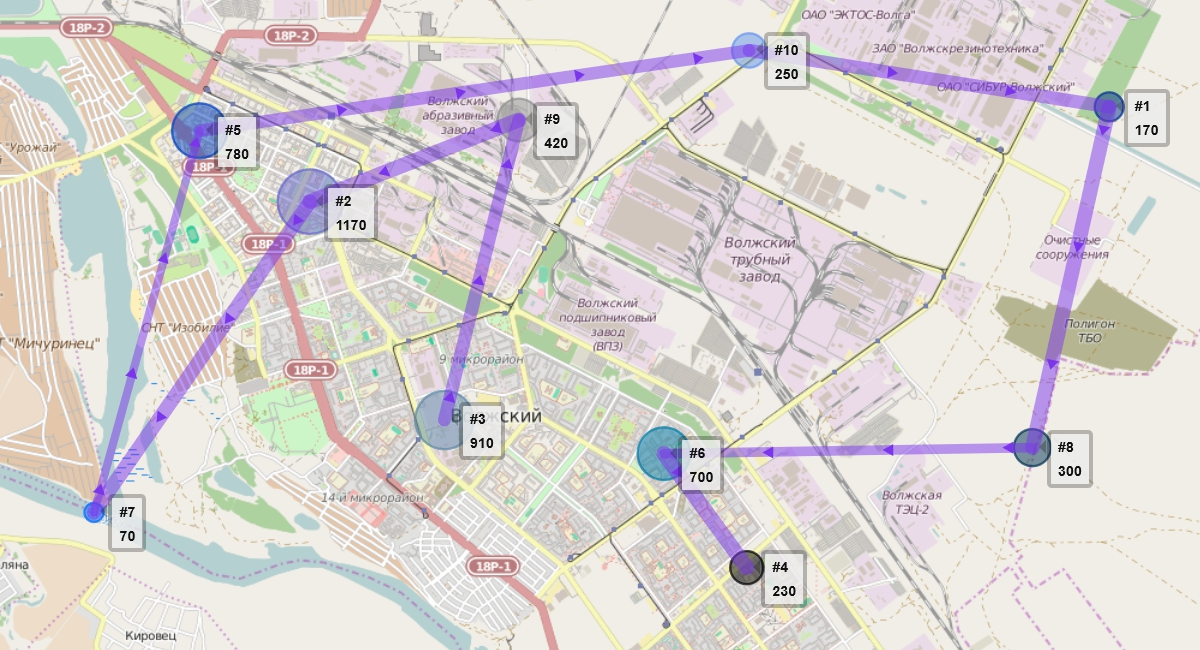
\includegraphics[width=\textwidth]{simulated-annealing-03}
    \caption{Полученый список обхода: \( 3, 9, 2, 7, 5, 10, 1, 8, 6, 4 \)\\
        Значение целевой функции: \( 0.0971 \)}
    \label{fig:sim-ann-01}
    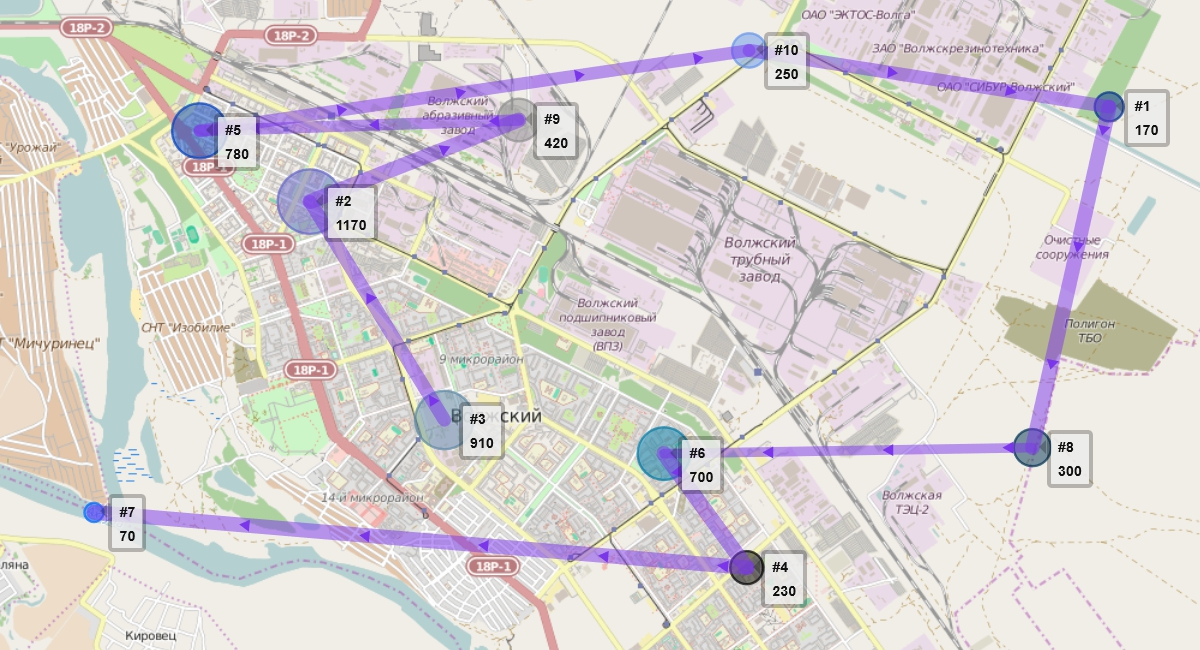
\includegraphics[width=\textwidth]{simulated-annealing-04}
    \caption{Полученый список обхода: \( 3, 2, 9, 5, 10, 1, 8, 6, 4, 7 \)\\
        Значение целевой функции: \( 0.0983 \)}
    \label{fig:sim-ann-02}
\end{figure}
\begin{figure}[ht!]
    \centering
    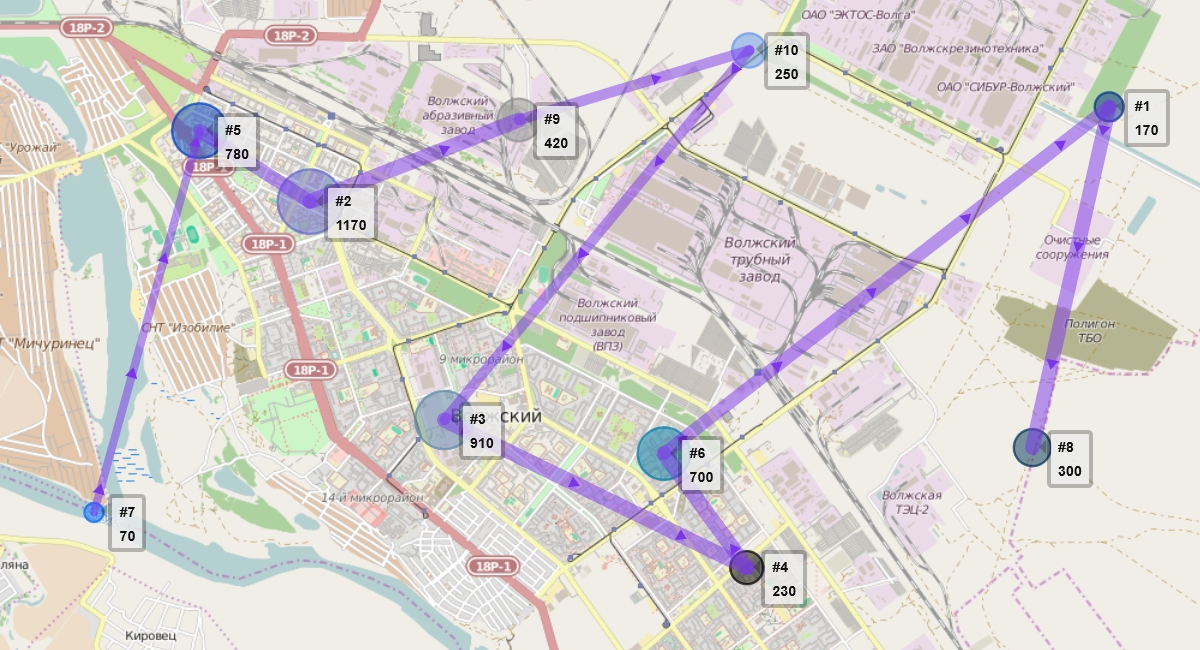
\includegraphics[width=\textwidth]{simulated-annealing-02}
    \caption{Полученый список обхода: \( 7, 5, 2, 9, 10, 3, 4, 6, 1, 8 \)\\
        Значение целевой функции: \( 0.1056 \)}
    \label{fig:sim-ann-03}
    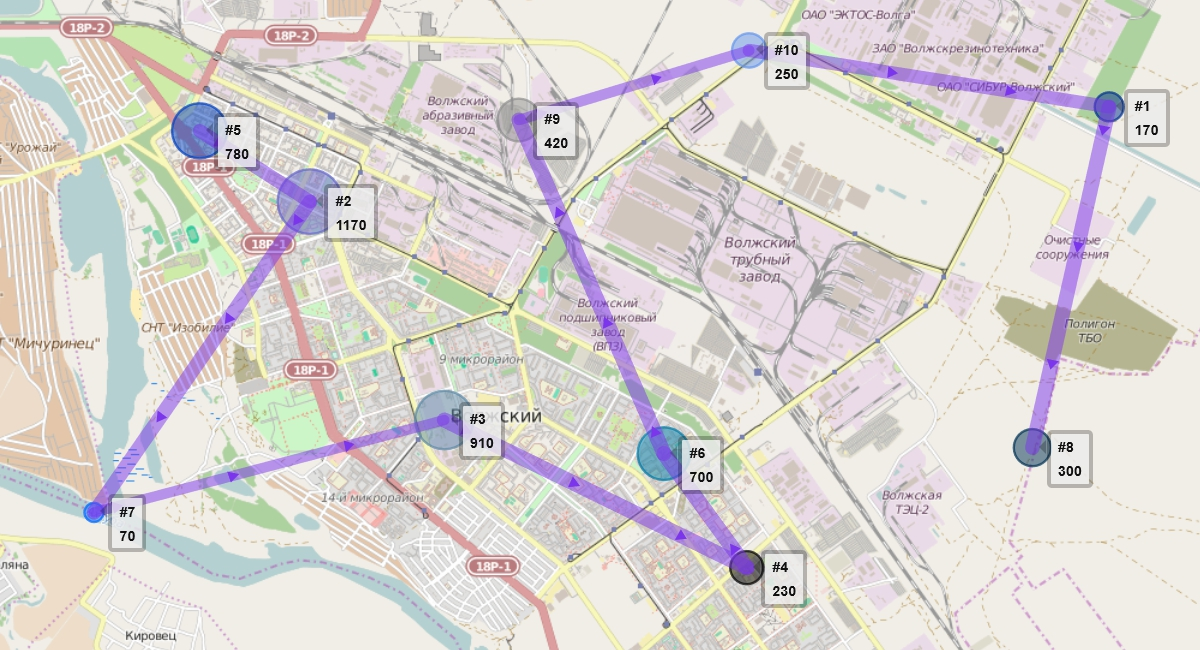
\includegraphics[width=\textwidth]{simulated-annealing-01}
    \caption{Полученый список обхода: \( 5, 2, 7, 3, 4, 6, 9, 10, 1, 8 \)\\
        Значение целевой функции: \( 0.1248 \)}
    \label{fig:sim-ann-04}
\end{figure}
\newpage

\subsection{Поиск с запретами}
Как и алгоритм имитации отжига, поиск с запретами является метаэвристикой, основанной на локальном поиске, 
где на каждой итерации выбирается лучшее решение в окрестности текущего решения в качестве нового текущего 
решения, даже если это приводит к увеличению стоимости решения.

Краткий анализ алгоритма:
\begin{itemize}
    \item лёгкая адаптация к сложным моделям;
    \item простота и возможность гибридизации с другими методами;
    \item возможность перехода между локальными оптимумами;
    \begin{itemize}
        \item использование списка запретов;
        \item хранение только \( l \) элементов списка;
    \end{itemize}
    \item выбор мер схожести для сравнения решений;
    \item вероятность \emph{застрять} в локальной окрестности;
\end{itemize}

\begin{algorithm}[ht!]
    \caption{Общий алгоритм поиска с запретами}
    \KwData{\( T \) -- длина списка запретов, \( N \) -- количество модификаций,\\
        \( A \) -- начальное решение}
    \KwResult{\( B \) -- результат алгоритма}
    \( l \leftarrow \) требуемая длина списка запретов \( T \)\;
    \( n \leftarrow \) количество модификаций \( N \)\;
    \( S \leftarrow \) начальное решение \( A \)\;
    \( B \leftarrow S \)\;
    \( L \leftarrow { S } \) список запретов длины \( l \) с записанным \( S \)\;
    \Repeat{достигнут предел по количеству итераций}{
        \If{Length(L) > l}{
            Удалить самый старый элемент из \( L \)\;
        }
        Выбрать решение \( R \) из \( S \)\;
        \For{n-1}{
            Выбрать решение \( W \) из \( S \)\;
            \If{\( W \notin L \) и \( (f(W) > f(R) \) или \( R \in L) \)}{
                \( R \leftarrow W \)\;
            }
            \If{\( R \notin L \) и \( f(R) > f(S) \)}{
                \( S \leftarrow R \)\;
                Записать \( R \) в \( L \)\;
            }
        }
        \If{\( f(S) > f(B) \)}{
            \( B \leftarrow S \)\;
        }
    }
    \label{alg:tabu-search}
\end{algorithm}

\emph{Основная проблема:} необходимо введение параметра отвечающий за число итерация, для предотвращения 
зацикливаний алгоритма.

\subsection{Семейство генетических алгоритмов}
Генетический алгоритм -- это эвристический алгоритм поиска, используемый для решения задач оптимизации и 
моделирования путём случайного подбора, комбинирования и вариации искомых параметров с использованием 
механизмов, аналогичных естественному отбору в природе. Является разновидностью эволюционных вычислений, 
с помощью которых решаются оптимизационные задачи с использованием методов естественной эволюции, таких 
как наследование, мутации, отбор и кроссинговер. Отличительной особенностью генетического алгоритма 
является акцент на использование оператора <<скрещивания>>, который производит операцию рекомбинации 
решений-кандидатов, роль которой аналогична роли скрещивания в живой природе.

Краткий анализ алгоритма:
\begin{itemize}
    \item кодирование информации в виде хромосом;
    \item использование операций скрещивания, селекции и мутации;
    \item реализация операций в задаче коммивояжера.
\end{itemize}

\begin{algorithm}[ht!]
    \caption{Общий вид генетического алгоритма}
    1. \emph{Инициализация}: порождение начальной популяции\;
    2. \emph{Выбор окрестности}: выбор операторов \emph{crossover} и \emph{mutation}\;
    3. \emph{Выбор родителя}: использование оператора селекции к текущей популяции\;
    4. \emph{Реализация шага}: использование операторов \emph{crossover}, 
        \emph{mutation}, \emph{hill climbing}, выбора потомка и родителя для получения 
        новой популяции\;
    5. Если критерии остановки не выполняются перейти к шагу 3 (продолжить эволюцию) 
        или перейти к шагу 1-3 (изменить критерии эволюции)\;
    \label{alg:genetic}
\end{algorithm}

\emph{Основная проблема:} представление графа сети в виде хромосом.

\clearpage

\subsection{Жадный алгоритм}
\label{sec:greedy-alg}
\subsubsection{Общее описание}
Поглощающий алгоритм (<<жадный алгоритм>>) -- тип алгоритмов оптимизации, которые на каждом шаге выбирают 
локально оптимальную альтернативу приносящую на этом шаге максимальную выгоду. Работают быстро, но обычно 
дают глобально неоптимальное решение, так как пропускают случай, когда лучше на данном шаге выбрать не самую 
лучшую альтернативу, но затем на следующем шаге получить значительный выигрыш.

Входные данные: полносвязный граф, в котором вершины заданы географическими координатами и количеством 
точек отправления или назначения в кластере, а рёбрам предписаны веса означающие потребность в перевозке 
пассажиров между кластерами. Это может быть, например, количество необходимых перевозок в час в то или иное 
время суток (например, в часы пик или же наоборот в спокойное время).

В результате кластеризации исходных данных на предыдущем этапе получен полносвязный граф, вершины 
которого -- центры кластеров (заданы географическими координатами и количеством точек отправления или 
назначения в кластере). Веса рёбер -- потребность в перевозке пассажиров между кластерами. 

\subsubsection{Схематическое представление}
Последовательность работы алгоритма описывается следующими шагами:
\begin{enumerate}
    \item определяем ребро графа с максимальной потребностью в транспорте;
    \item выбираем из двух вершин, которые это ребро соединяет, одну, с максимальным количеством 
        пассажиров в ней;
    \item делаем первый шаг из этой вершины в другую, выбирая то ребро, которое имеет максимальную 
        потребность;
    \item из этой вершины делаем шаг в следующую, тоже выбирая ребро с максимальной потребностью:
    \begin{enumerate}
        \item если два ребра имеют одинаковую пропускную способность, то выбираем любое;
        \item если ребро имеется в списке, то выбираем следующее по пропускной способности;
    \end{enumerate}
    \item строим до тех пор, пока длина маршрута не превысит пороговое значение;
    \item переходим к пункту 1, выбрав следующее по пропускной способности ребро.
\end{enumerate}

\subsubsection{Результат работы}
Пример работы алгоритма приведен на рисунке \ref{img:greedy-01}.
\begin{enumerate}
    \item Выбираем ребро с потребностью перевозки 300.
    \item Выбираем кластер с количеством точек 500.
    \item Первый шаг: начинаем маршрут с ребра 300.
    \item Второй шаг: выбираем ребро 200.
    \item Третий шаг: выбираем ребро 100.
\end{enumerate}

\begin{figure}[h!]
    \centering
    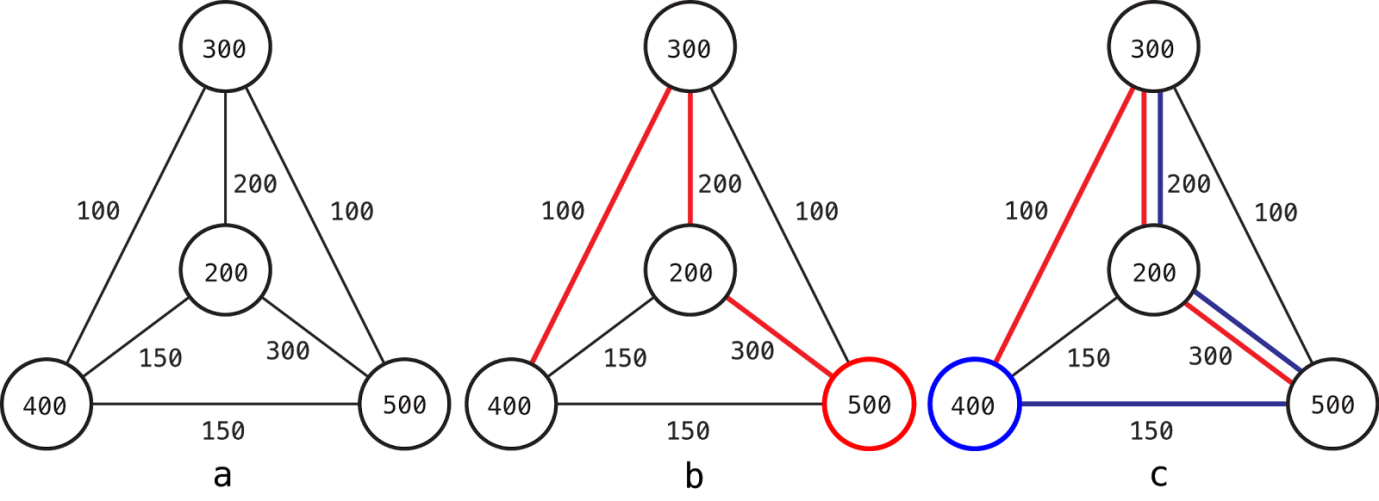
\includegraphics[width=0.8\textwidth]{greedy-01}
    \caption{Пример реализации алгоритма\\
        a -- исходный граф;\\
        b -- первый построенный маршрут (вершина начала пути выделена красным);\\
        c -- второй построенный маршрут (вершина начала пути выделена синим).
    }
   \label{img:greedy-01}
\end{figure}

\section{Алгоритм минимального увеличения длины}
\label{sec:second_alg}
\subsection{Общее описание}
Формирование начальной сети маршрутов, используя принцип <<минимального>> увеличения длины маршрута при 
включении нового пункта. Идея алгоритма заключается в итеративном добавлении в существующие маршруты узлы, 
минимально увеличивающие длину исходных маршрутов. 

На вход алгоритма подаются: \( n_r \) -- число маршрутов в сети, \( N_c \) –- число узлов 
(центров кластеров), \( C_t \) – множество терминальных узлов (определенных посредством построения 
окружности, содержащей все узлы), \( C_{nt} \) -- множество нетерминальных узлов (сумма элементов множества 
терминальных и нетерминальных узлов равна числу центров кластера), матрица длин размером 
\( ||{C_{nt}} + {C_{t}}|| \times ||{C_{nt}} + {C_{t}}|| \). Заметим, что \( C_t + C_{nt} = n_c \)

Выходом алгоритма является транспортная сеть \( R_i \), содержащие непересекающиеся множество узлов, 
\( r_{i} = [p_{1}^{(i)}, \dots, p_{k}^{(i)}] \), где \( i = 1, \dots, n_r \). 

Псевдокод алгоритма представлен следующей схемой \ref{alg:min-length}.
\begin{algorithm}[ht!]
    \caption{Алгоритм построения маршрутной сети}
    \KwData{\( n_r, C_t, C_nt \)}
    \KwResult{\( R_i \) -- список маршрутов сети.}
    1. Создать сеть Ri соединяющий вершины Ct\;
    2. \For{Для каждого i-го маршрута из сети Ri выполнить}{
        1. Поместить вершины маршрута (попарно) в список \( PN \)\;
        2. Найти вершину \( c_j \), присоединение которой минимально увеличивает длину маршрута из 
            \( PN \) и добавить новый маршрут в список \( RC \)\;
        3. Составить новый список \( RCC \) состоящий из маршрутов, полученных путём замены пар 
            вершин \( PN \) на изменённые \( RC \)\;
        4. Рассчитать длины маршрутов в списке RCC, используя OSRM\;
        5. Выбрать из \( RCC \) маршрут \( R^{\star}_i \) с минимальной длиной\;
        6. Заменить \( R_i \) на \( R^{\star}_i \)\;
        7. Удалить узел \( c_j \) из \( C_{nt} \) добавленный в \( R^{\star}_i \)\;
    }
    3. Если список \( C_nt \) не пустой, перейти на шаг 2, иначе закончить построение\;
    \label{alg:min-length}
\end{algorithm}

\subsection{Объяснение работы}
Поясним работу данного алгоритма на простом примере. Имеем некоторый набор терминальных кластеров 
\( A, A', B, B' \) (\( C_t \)) и нетерминальных \( C, D, \) \( E, F \) (\( C_{nt} \)). Количество маршрутов 
для построения \( n_r = 2 \). Необходимо построить два маршрута на основе входных данных.

Первым шагом является определение прямых маршрутов, которые включают только терминальные узлы. Условимся, 
что для первоначального маршрута и используются противоположные узлы, то есть расположенные напротив друг 
друга. В данном случае получаем список содержащий два узла \( R_i = [AA', BB'] \). Рисунок 
\ref{fig:route_first} иллюстрирует данное начальное распределение маршрутов.

\begin{figure}[ht!]
    \centering
    \begin{subfigure}{0.3\textwidth}
        \centering
        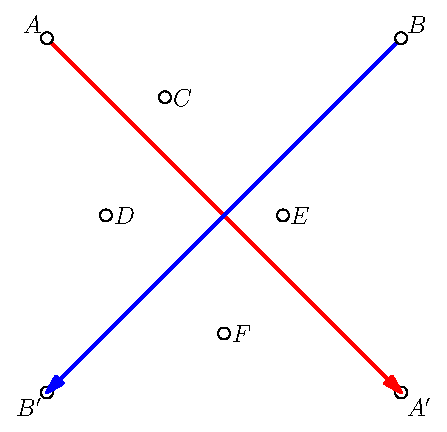
\includegraphics[width=\textwidth]{route01}
        \caption{Первоначальная маршрутная сеть включающая \( n_r \) прямых маршрутов с терминальными узлами.}
        \label{fig:route_first}
    \end{subfigure}
    \begin{subfigure}{0.3\textwidth}
        \centering
        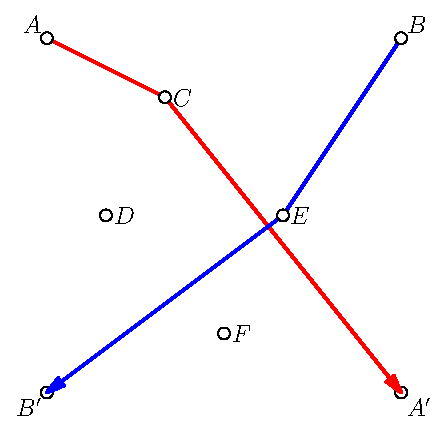
\includegraphics[width=\textwidth]{route02}
        \caption{Маршрутная сеть после первой итерации алгоритма.}
        \label{fig:route_second}
    \end{subfigure}
    \begin{subfigure}{0.3\textwidth}
        \centering
        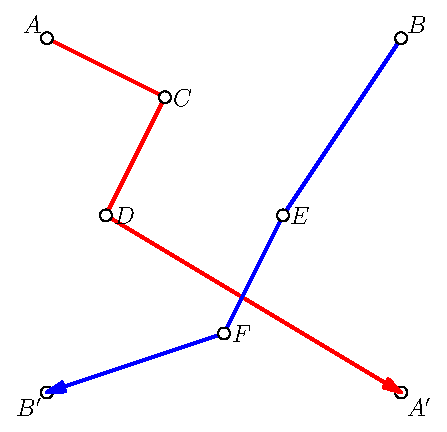
\includegraphics[width=\textwidth]{route03}
        \caption{Окончательная версия маршрутной сети.}
        \label{fig:route_third}
    \end{subfigure}
    \caption{Схематичное представление работы алгоритма}
    \label{fig:route}
\end{figure}

Далее, выбираем из первый элемент из списка \( R_i \) и разбиваем его на пары. На данном шаге, так как 
в маршруте только два узла, имеем только одну пару \( PN = [AA'] \).

Далее, конструируем набор маршрутов добавлением нового элемента в середину пары в существующие маршруты 
из \( PN \). В данном случае имеем следующий набор \( ACA', ADA', AEA', AFA' \).

Для полученных четырёх маршрутов рассчитаем длину для каждого и выбираем с наименьшим значением 
(в нашем случае это \( ACA' \)). Добавляем \( ACA' \) в список маршрутов \( RC = [ACA'] \).

Далее, составляем все варианты новых маршрутов из \( RC \) и \( PN \). В данном случае получаем только 
один \( ACA' \) и добавляем его в список \( R^{\star}_{i} \). Узел \( С \) удаляем из списка \( C_nt \).
Проделываем аналогичные действия и для второго маршрута -- получаем новый маршрут \( BEB’ \).
Рисунок \ref{fig:route_second} отражает маршрутную сеть после первой итерации алгоритма.

На второй итерации цикла имеем список маршрутов \( R_i = [ACA', BEB'] \). Используя \( ACA' \) можно 
сконструировать две пары \( PN=[AC, CA'] \).

Последовательно добавляя каждый нетерминальный кластер имеем следующий список \( ADC, AFC, CDA', CFA' \). 
Допустим, что минимальным из них является \( CDA' \).

Составляем различные варианты из \( CDA' \) и \( AC \), \( CA' \) получаем новый \( ACDA' \). Добавляем 
полученный маршрут в \( R^{\star}_i \) и удаляем узел \( D \) из \( C_nt \).

Аналогично для второго маршрута из \( R_i \) получаем \( BEFB' \).

Так как \( C_nt \) не содержит больше узлов (пустой список), то алгоритм заканчивает свою работу.

Рисунок \ref{fig:route_third} отражает окончательный этап алгоритма.

\subsection{Использование алгоритма выпуклой оболочки}
Определим полносвязанный граф G, вершины которого -- центры построенных на предыдущем шаге кластеров. 
Веса вершин графа -- количество корреспонденций которые осуществляют жители из данной вершины. Веса 
ребер -- объем корреспонденций между вершинами.

Для поиска узлов отправления-назначения, для начальной сети прямых маршрутов (шаг 1), используется простая 
идея основанная на идее алгоритма выпуклой оболочки.

Для всех заданных узлов создаётся выпуклая оболочка. Это помогает нарисовать круг описанный вокруг данной
оболочки. Так как у нас есть ряд маршрутов в качестве входного параметра, то определяем \( 2\cdot n_r \) 
равномерно расположенных узлов на построенной окружности. Узлы расположенные напротив друг друга являются 
квази-узлами отправления/назначения для маршрутной сети. Для определения реального узла отправления/назначения 
выбираем вокруг квази-узла некоторый \( \varepsilon \) радиус и находим все принадлежащее узлы к данной 
окрестности.Так как список может попасть больше чем один узел, то необходимо произвести сортировку данных 
узлов по количеству людей находящимся в нём и выбирать с наибольшим количеством. Псевдокод алгоритма 
представлен схемой \ref{alg:convex-hull}.

\begin{algorithm}[ht!]
    \caption{Алгоритм формирования узлов отправления-назначения}
    \KwData{\( nr \) -- количество маршрутов для построения (подбирается с учетом конкретной задачи), 
        \( G \) -- список вершин исходного графа.}
    \KwResult{\( C_t \) -- список терминальных вершин, \( Cnt \) -- список нетерминальных вершин.}
    1. Рассчитать координаты центра \( r_0 \) окружности, охватывающей все вершины графа G (складываем 
        покомпонентно координаты узлов и делим полученные значения на количество узлов)\;
    2. Сформировать список \( D \) расстояний от \( r_0 \) до каждой вершины \( c_j \)\;
    3. Найти вершину с максимальным удалением от центра окружности и построить окружность с радиусом 
        равным расстоянию до этой вершины\;
    4. Разбить окружность на \( 2\cdot n_r \) равных отрезков и поместить значения полученных 
        углов (в полярной системе координат) в \( N_c \)\;
    5. Обойти список \( N_c \) и получить координаты точек на окружности по углу и радиусу с 
        использованием проекции Меркатора, и поместить полученные значения координат вершин в 
        список \( C_t \)\;
    \For{Для каждой вершины \( c_j \) из \( C_t \)}{
        1. Найти узлы в окрестности \( \varepsilon \), добавить в список \( T \)\;
        2. Выбрать из списка \( T \) вершину \( c_k \) с максимальным весом\;
        3. Заменить \( c_j \) на \( c_k \)\;
    }
    7. Составить список \( C_{nt} \) из вершин не входящих в список Ct\;
\end{algorithm}

\subsection{Результаты работы}
Алгоритм был апробирован на различных тестовых данных для различных значений числа маршрутов. 
Результат работы алгоритма представлен на \ref{img:min-length-01}.
\begin{figure}[h!]
    \centering
    \begin{subfigure}{0.75\textwidth}
        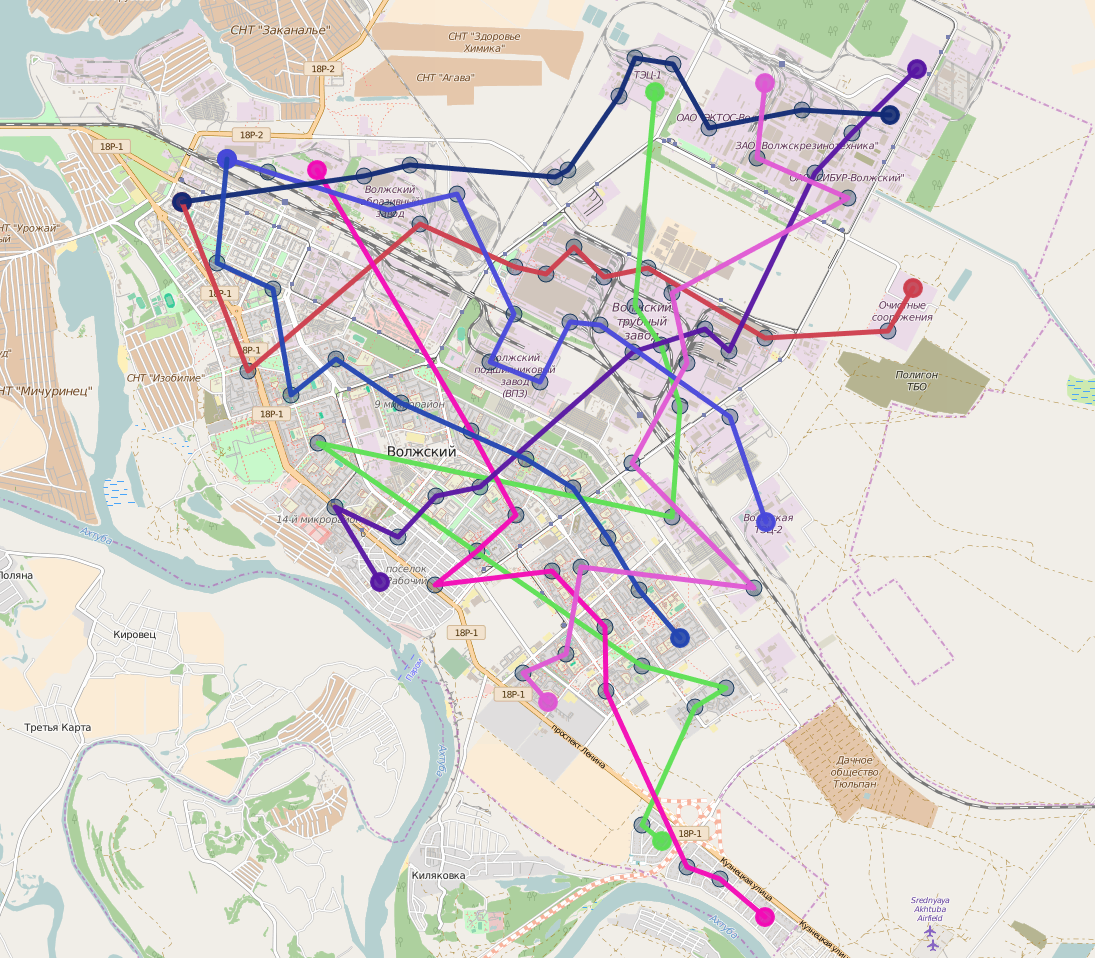
\includegraphics[width=\textwidth]{minimal-01}
        \caption{Построением маршрута по графу}
        \label{fig:graph}
    \end{subfigure}
    \begin{subfigure}{0.75\textwidth}
        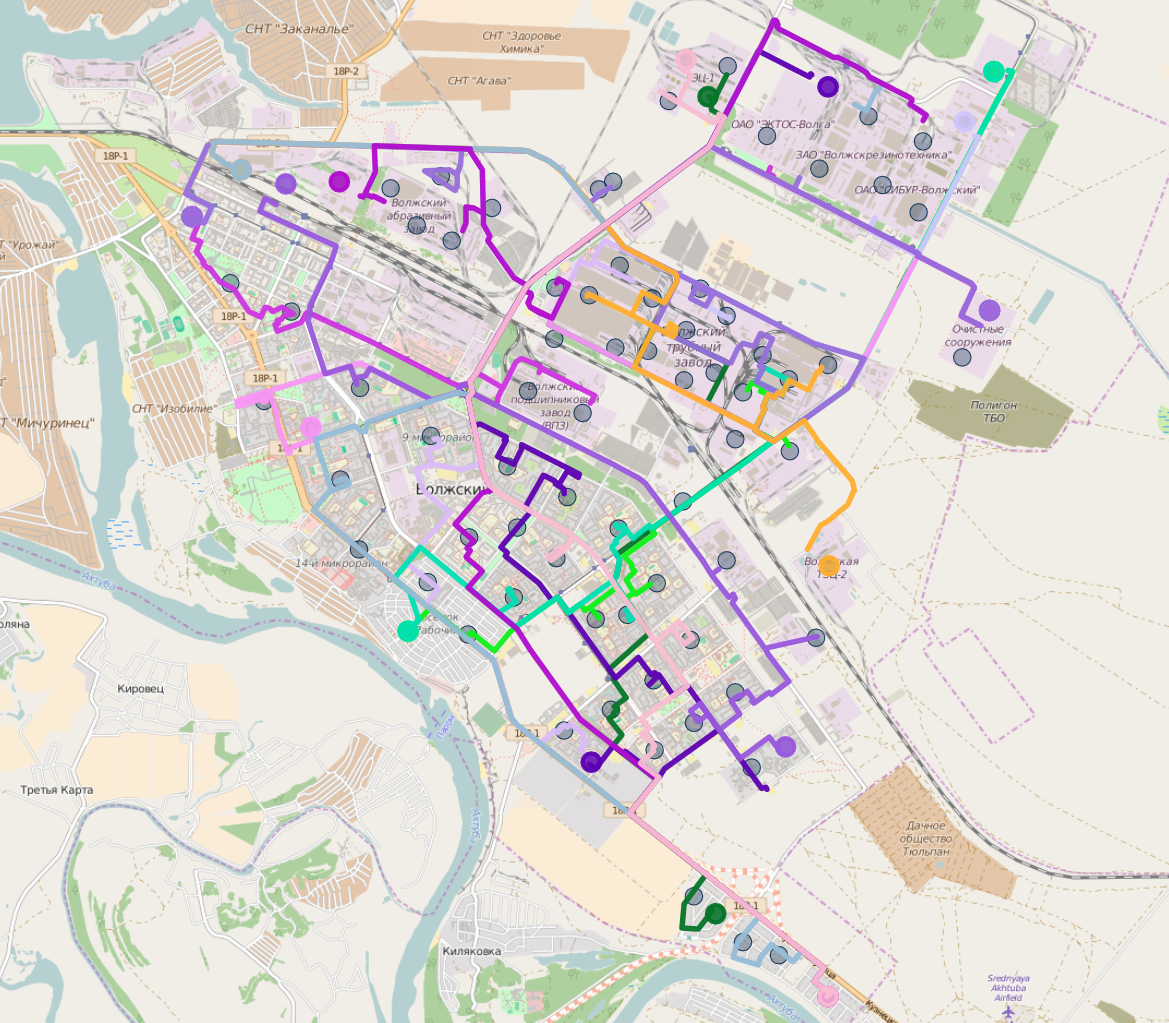
\includegraphics[width=\textwidth]{minimal-02}
        \caption{Построением маршрута по дорогам}
        \label{fig:osrm}
    \end{subfigure}
    \caption{Визуализация результата работы алгоритма формирования начальной сети маршрутов, 
        использующий принцип <<минимального>> увеличения длины маршрута при включении нового пункта%:\\
        % a -- с построением маршрута по графу\\
        % b -- с построением маршрута по дорогам
    }
   \label{img:min-length-01}
\end{figure}

\clearpage

\section{Алгоритм модификации начальной сети маршрутов}
\label{sec:third-alg}
% ---------------
% 3 метод -- WIP
% ---------------
\emph{Модификация начального варианта сети маршрутов общественного транспорта с целью минимизации функции 
затрат и генерация вариантов альтернатив сетей}
\subsection{Общее описание}
Модификация начального варианта сети маршрутов общественного транспорта осуществляется с использованием идеи 
итерационного эволюционного преобразования исходного маршрута. Предлагается эволюционный алгоритм, 
использующий операции мутации и кроссовера для оптимизации длины сети маршрутов.

\subsection{Идея метода}
Эволюционный алгоритм представлен следующей последовательностью шагов. 
\begin{enumerate}
    \item[1.] Если выбрана стратегия формирования единственного начального маршрута, то 
    \begin{enumerate}
        \item[1.1.] Сформировать единственный маршрут жадным алгоритмом.
        \item[1.2.] Разрезать маршрут на \( k \) маршрутов (где \( k \) -- изначально заданное число 
            маршрутов).
    \end{enumerate}
    \item[2.] Если выбрана стратегия формирования начальной сети, то перейти на шаг 3.
    \item[3.] Оценить качество сети маршрутов (с использованием критериев качества, например длины 
        маршрутной сети).
    \item[4.] Применить операцию кроссовера и мутации для получения новой генерации транспортной 
        сети \cite{bib:20}.
    \begin{enumerate}
        \item[4.1.] Оценить качество новой сети маршрутов.
        \item[4.2.] Если новая популяция лучше предыдущей, сохранить ее.
        \item[4.3.] Если новая популяция хуже предыдущей, отклонить. 
    \end{enumerate}
    \item[5.] Повторить, пока не выполняется условие останова.
\end{enumerate}

\subsection{Схематическое представление}
\subsection{Результаты работы}

\section{Заключение}
    \chapter{Испытание и обоснование эффективности предлагаемых подходов}
\section{Проектирование ПО}
Разработанное программное обеспечение дожно соответствовать техническому заданию представленное в Приложении 
А и должна обеспечивать возможность выполнения следующих ниже функций:
\begin{enumerate}
    \item Предоставлять возможность сохранять и загружать данные используемые для работы программы:
    \begin{itemize}
        \item загрузка кластеризованных данных о перемещении;
        \item преобразование загруженных данных во внутренний формат программы;
        \item сохранения расчётных данных для последующей обработки;
    \end{itemize}
    \item Предоставлять возможность по построению матрицы корреспонденций по данным о перемещении для 
        для последующего построения транспортной сети.
    \item Предоставлять возможность анализа графа корреспонденций для выбора узлов отправления-назначения для 
        последующего построения транспортной сети.
    \item Предоставлять функцию построения маршрутной сети по заданным параметрам, включающая следующие 
        пункты:
    \begin{itemize}
        \item инициализации первичной маршрутной сети;
        \item построения маршрутной сети по заданной метрике;
        \item модификация маршрутной сети;
        \item взаимодействие с программных обеспечение OSRM;
    \end{itemize}
    \item Предоставлять возможность производить оценку построенной маршрутной сети, по следующим критериям:
    \begin{itemize}
        \item оценка маршрута по критерию (длина, количество пассажиров и т.~п.);
        \item общая оценка маршрутной сети;
        \item многокритериальная оценка.
    \end{itemize}
\end{enumerate}

Подробности по проектировнию ПО описаны в Приложении А. Рассмотренные алгоритмы из главы \ref{chp:methods} 
были реализованы с использованием языка программирования Python и сервиса построения маршрутов Open Source 
Routing Machine (OSRM) для расчёта расстояния между узлами графа по городским дорогам. Программный код 
опубликован на хостинге Github (подробнее в Приложении В).

\section{Методика проведения эксперимента}
Для оценки эффективности алгоритма и изучения его специфики, были проведены эксперименты в ходе которых 
менялось количество узлов в дорожном графе и количество создаваемых маршрутов в городской сети, а также 
несколько вариантов реализации данного метода. Наиболее интересным случаем является, когда обрабатывается 
большое число узлов в графе или большое число геопространственных данных.

Были сгенерированы данных о предпочтениях по перемещению жителей среднего по размерам города с примерным 
числом жителей около 350 000. В качестве результата, было получено 6000 пар точек отправления-назначения или 
12000 точек в общей сложности. Матрица корреспонденций в данном случае имеет очень большой размер 
\( 6000 \times 6000 \) элементов, где элемент с индексом \( i, j \) имеет значение \( 0 \) -- отсутствие связи 
между \( i \)-ой и \( j \)-ой точкой, а \( 1 \) соответственно связь.

Для того, чтобы уменьшить размер матрицы корреспонденций и понять наиболее густонаселённые места, был 
применён алгоритм кластеризации точек отправления-назначения, который не входит в рассмотрение в данной 
работе.

Для того чтобы понять какое количество кластеров (или узлов) влияет на эффективность работы предложенного 
алгоритма было предложено произвести варьирование параметров: количество кластеров и количество маршрутов для 
построения.

Критериями для оценки эффективности разработанных алгоритмов является:
\begin{itemize}
    \item время затрачивание на расчёт;
    \item длина полученной маршрутной сети.
\end{itemize}

\chapter{Методология и результаты}
\section{Проведение эксперимента и описание результатов}
По мере того как количество кластеров изменяется получаем различные варианты производительности алгоритма. 
В проводимых экспериментах число узлов изменяется в диапазоне от 100 до 300.

Количество маршрутов для построения так же влияет на скорость работы предложенного алгоритма. Очевидно, что 
минимальное количество маршрутов определяется числом пар терминальных маршрутов. В данном случае варьирование 
числа маршрутов было произведено в интервале от 8 до 100 в зависимости от количества узлов.

В эксперименте использовалось эмпирическое правило, что число узлов должно быть в 20 раз больше, чем число 
маршрутов. Для упрощения оценки производительности применяется общая длина сети в качестве критерия качества.
Поскольку эта оценка производится во внешнем цикле, то она не имеет большого влияния на выполнение алгоритма.
Кроме того не была использована информация о возможных пробках влияющая на процедуру выбора соответствующего 
узла.

Чтобы понять эффективность работы алгоритма в зависимости от окружающей среды, были разработаны три 
альтернативных реализации:
\begin{enumerate}
    \item Последовательная реализация (или graph) алгоритма основанного на графе дорог. В данной реализации 
        предполагается, что связь между узлами может быть проведена по прямой линии, несмотря на состояние 
        дорог. Эту реализацию можно рассматривать в качестве базовой.
    \item Последовательная реализация с использованием OSRM (или S.OSRM) -- это усовершенствованная версия 
        предыдущей стратегии, где расстояние между кластерами рассчитывается с использование движка 
        маршрутизации OSRM по дорожной сети.
    \item Параллельная версия с использованием OSRM (или P.OSRM) предполагает возможность в распараллеливании 
        внутреннего цикла алгоритма.  
\end{enumerate}

\clearpage

\subsection{Последовательная реализация}
Данная реализация является наиболее простой из всех с точки зрения расчёта расстояния. В данном случае 
применяется евклидово расстояние между узлами с использованием проекции Меркатора. Эта версия может быть 
интересна в качестве ориентира в тесте производительности.

Однако стоит учесть что данная реализация не предназначена для использования на практики из-за того что не 
принимает во внимание естественные и искусственные препятствия, а также изменчивость в городской структуре.

Данная реализация представлена на рисунках \ref{fig:network-01a}, \ref{fig:network-01b} и 
\ref{fig:network-01c} как результат работы алгоритма на 100 узлах для 8 маршрутов, 200 узлах для 10 маршрутов 
и 300 узлах для 18 маршрутах соответственно. По таблице \ref{table-time-results} можно видеть, что для нескольких 
узлов (до 100) показывающие слабое влияние на время выполнения программы.

\subsection{Последовательная с использованием OSRM}
Последовательная реализация алгоритма является усовершенствованной версией предыдущей стратегии построения 
маршрутной сети, где расстояние между узлами графа рассчитывается с использование программного обеспечения 
Open Source Routing Machine (OSRM). Каждый раз когда алгоритму необходимой расчитать маршрут от одного узла 
до другого, то производит запрос к данному движку маршрутизации. Использование OSRM, для данной реализации, 
является узким местом, так как на обработку одного запроса тратится не менее 10 мс, а запросы производятся.

\subsection{Параллельная с использованием OSRM}
Для ускорения алгоритма \ref{alg:min-length} предлагается к распараллеливанию внутрений цикл (шаги 4-5).
Распараллеливание можно произвести, так как обработка происходит по независимым друг от друга парам узлов 
графа. Также используемый в работе сервис OSRM поддерживает многопоточную обработку запросов на построение 
маршрута, что также является плюсом данной реализации. 

Для реализации была использована асинхронная модель с использованием восьми потоков.

Данная реализация представлена на рисунках \ref{fig:network-02a}, \ref{fig:network-02b} и 
\ref{fig:network-02c} как результат работы алгоритма на 100 узлах для 14 маршрутов, 200 узлах для 12 маршрутов 
и 300 узлах для 16 маршрутах соответственно.

\subsection{Результаты}
Результаты эксперимента представлены на рисунках \ref{fig:result-01} и \ref{fig:result-02}, а также в таблице 
\ref{table-time-results}. Рисунки представлены в логарифмической шкале по оси ординат, для более удобного анализа 
полученных результатов. Построенные маршрутные сети представлены на рисунках \ref{fig:network-01a} -- 
\ref{fig:network-02c}. 

Остальные результаты доступны по ссылкам представленые в Приложении В.

\begin{figure}[ht!]
    \centering
    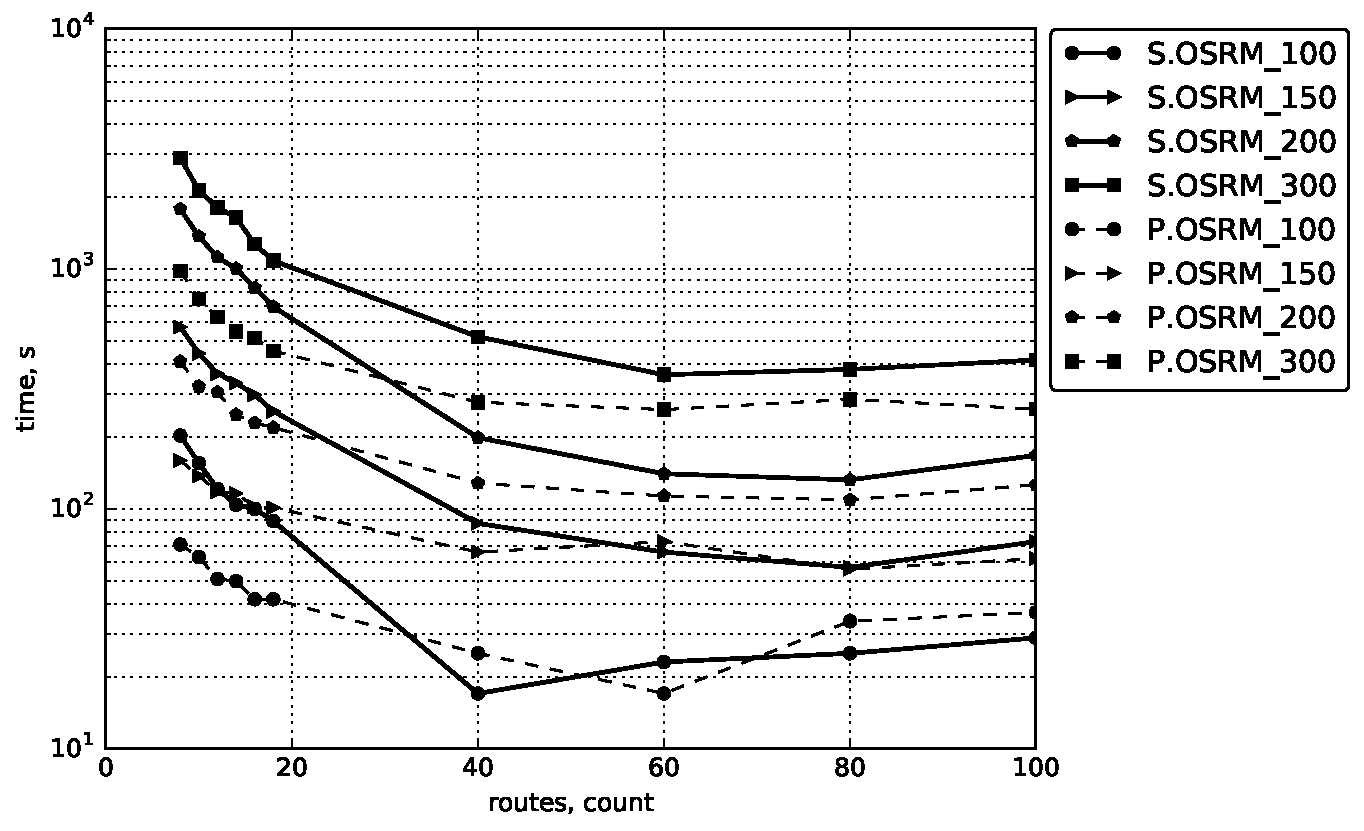
\includegraphics[width=\textwidth]{result-01}
    \caption{Зависимость времени построения от количества маршрутов}
    \label{fig:result-01}
\end{figure}

\begin{figure}[ht!]
    \centering
    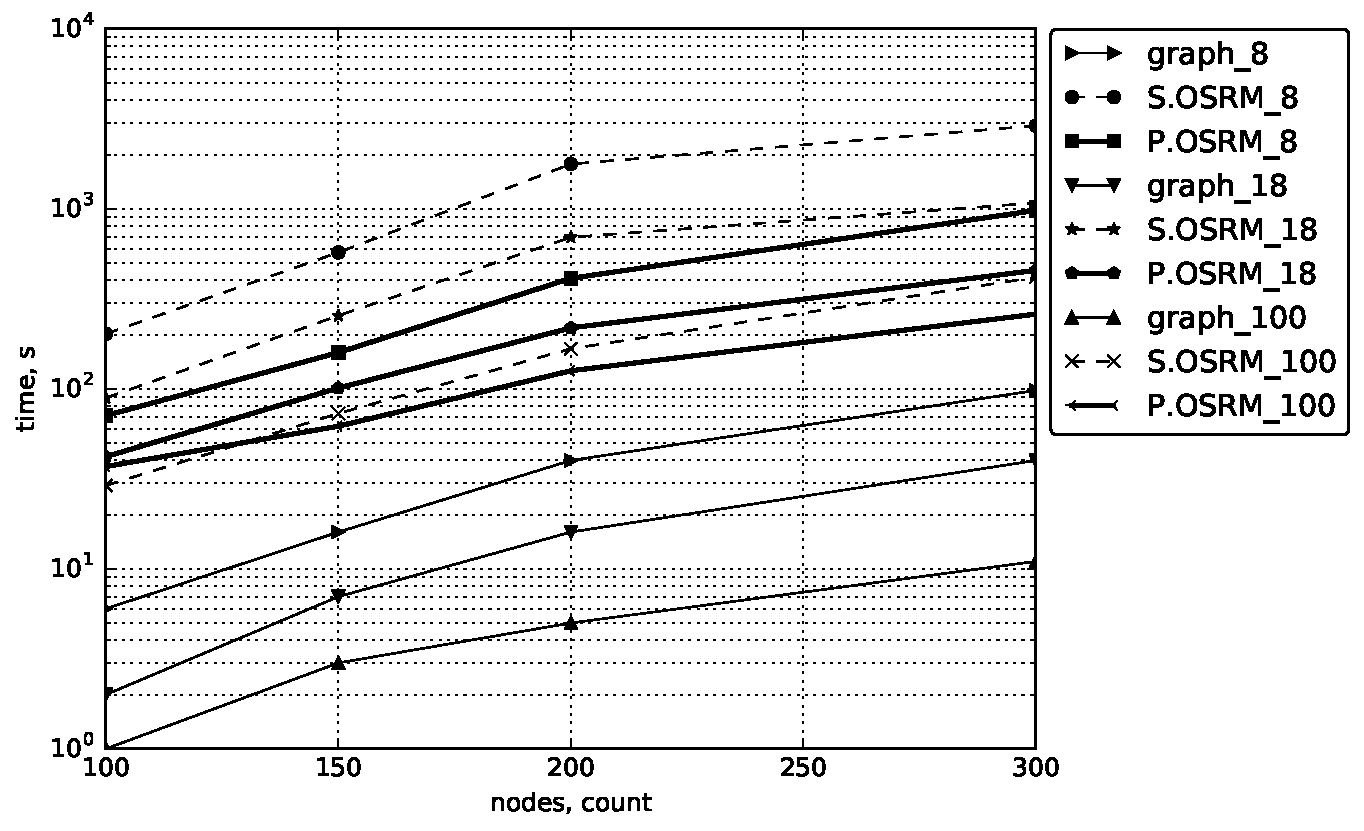
\includegraphics[width=\textwidth]{result-02}
    \caption{Зависимость времени построения от кластеров}
    \label{fig:result-02}
\end{figure}

\begin{figure}[ht!]
    \centering
    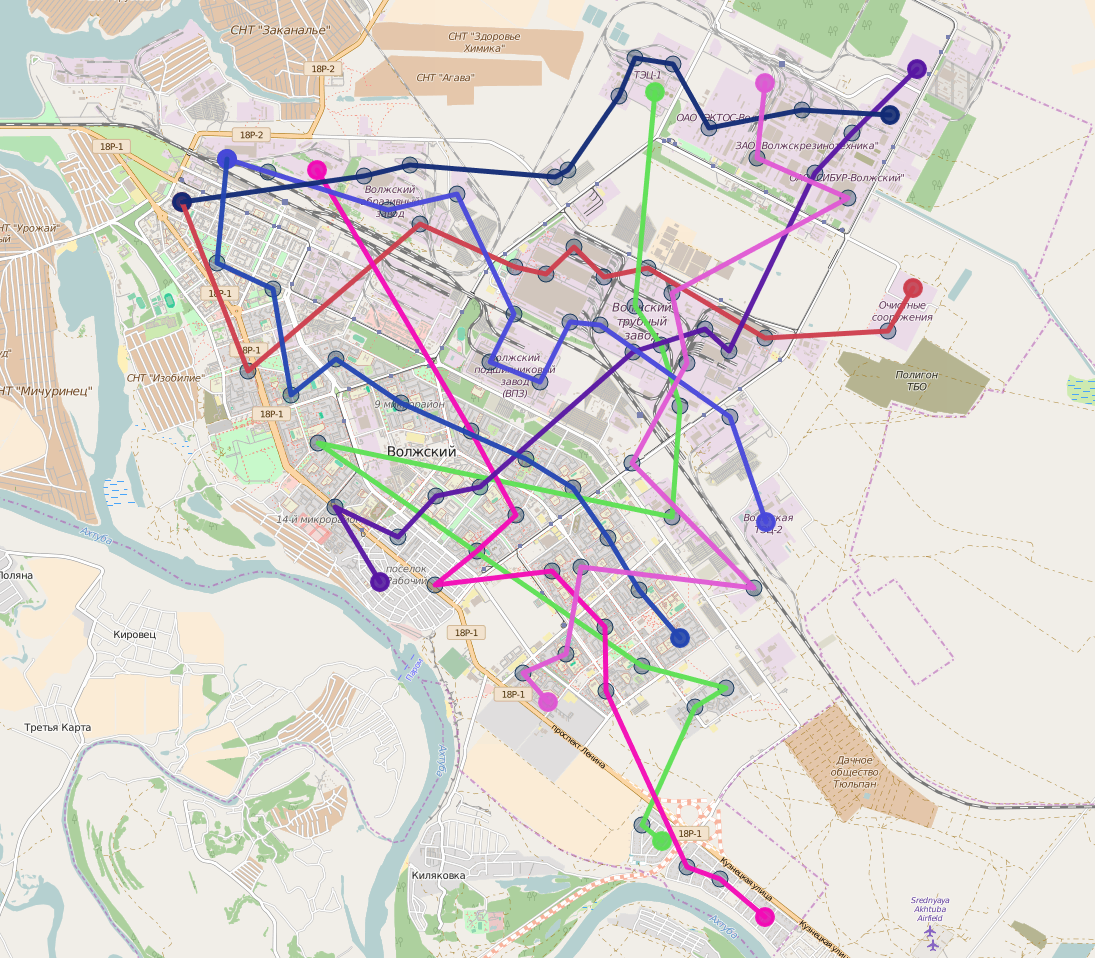
\includegraphics[width=0.8\textwidth]{100-8}
    \caption{Использование метрики graph для 100 кластеров и 8 маршрутов.}
    \label{fig:network-01a}
\end{figure}

\begin{figure}[ht!]
    \centering
    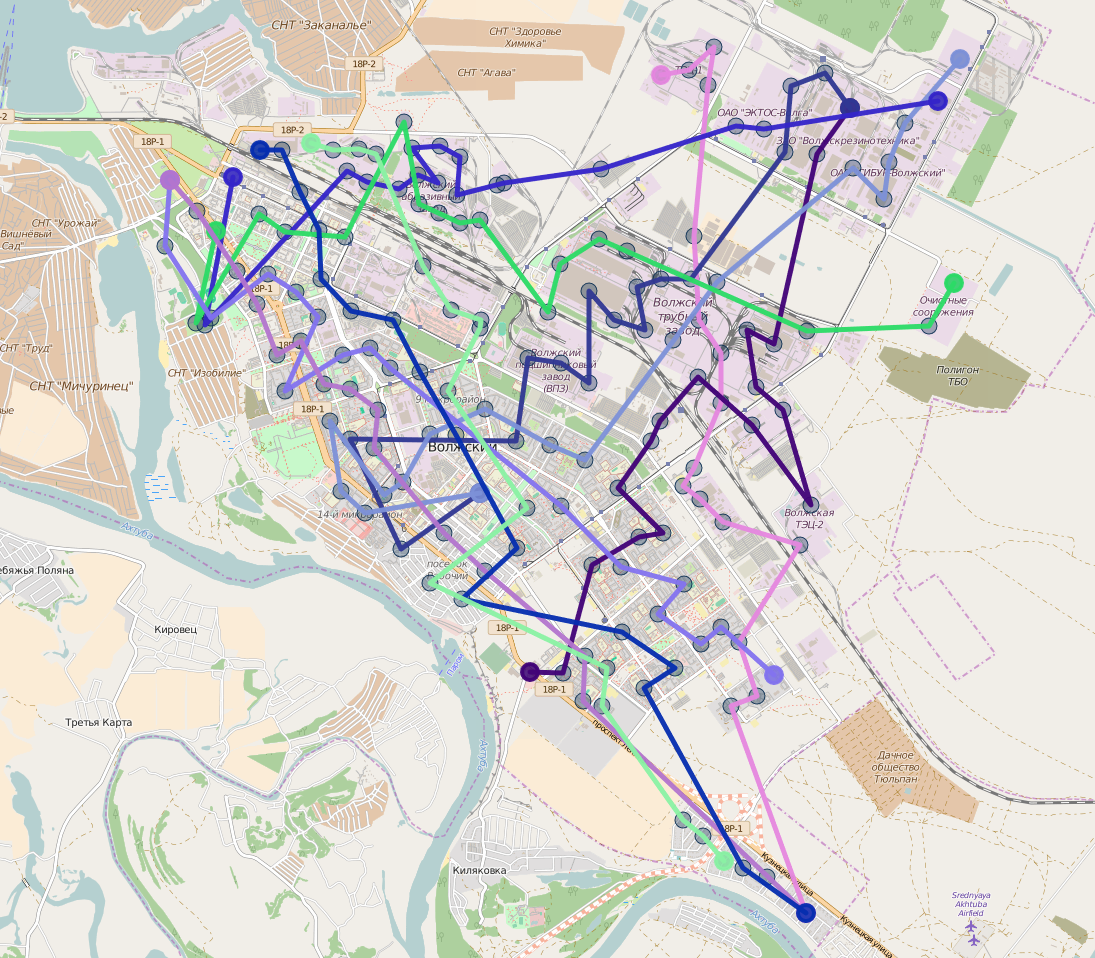
\includegraphics[width=0.8\textwidth]{200-10}
    \caption{Использование метрики graph для 200 кластеров и 10 маршрутов.}
    \label{fig:network-01b}
\end{figure}

\begin{figure}[ht!]
    \centering
    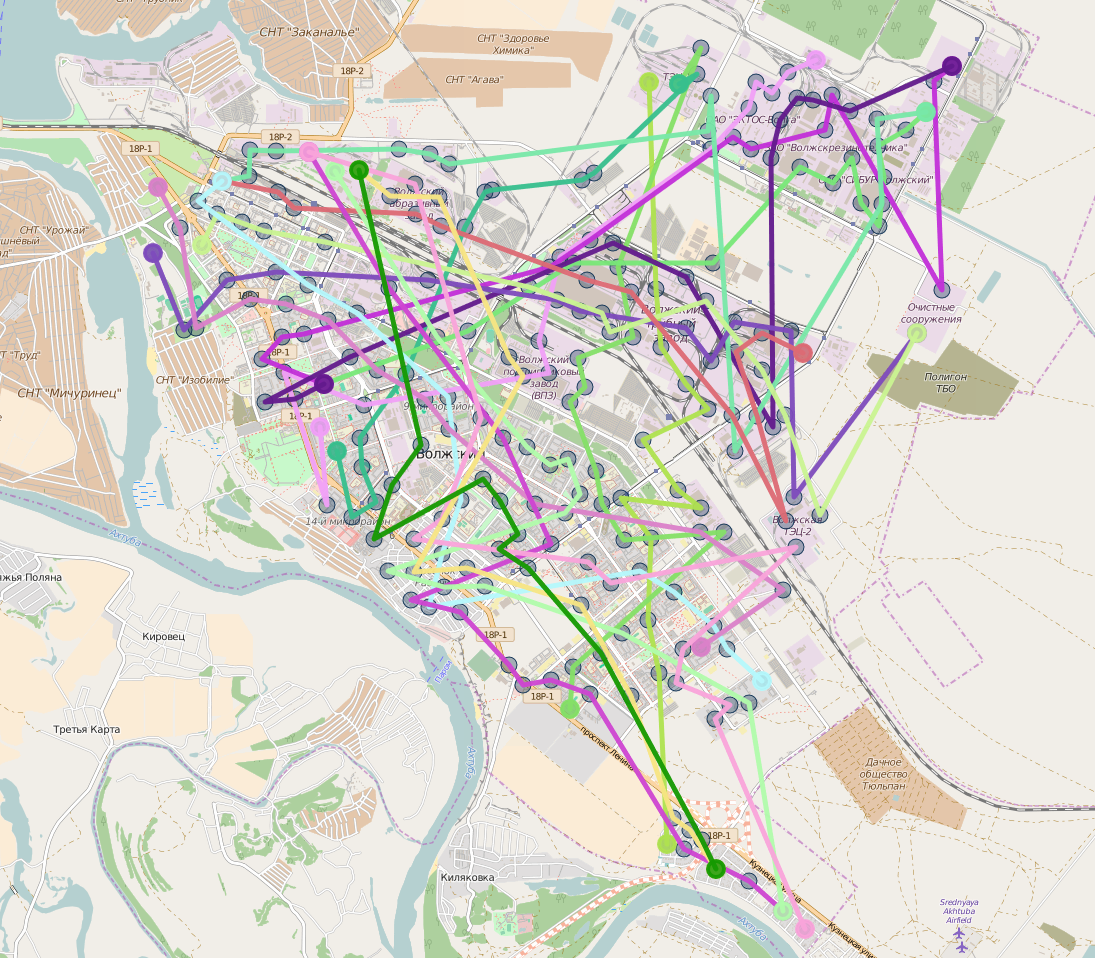
\includegraphics[width=0.8\textwidth]{300-18}
    \caption{Использование метрики graph для 300 кластеров и 18 маршрутов.}
    \label{fig:network-01c}
\end{figure}

\begin{figure}[ht!]
    \centering
    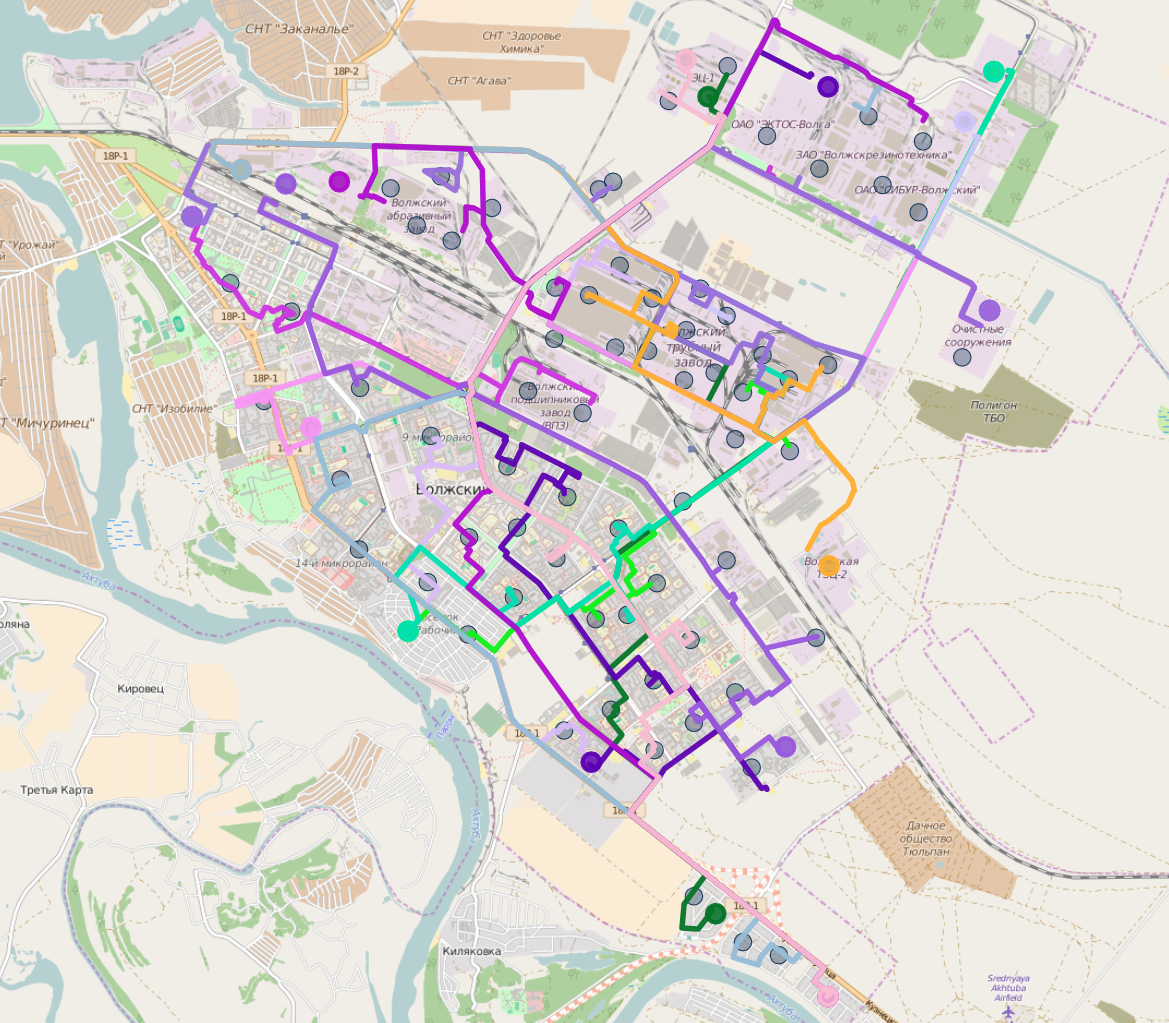
\includegraphics[width=0.8\textwidth]{100-14}
    \caption{Использование метрики OSRM для 100 кластеров и 14 маршрутов.}
    \label{fig:network-02a}
\end{figure}

\begin{figure}[ht!]
    \centering
    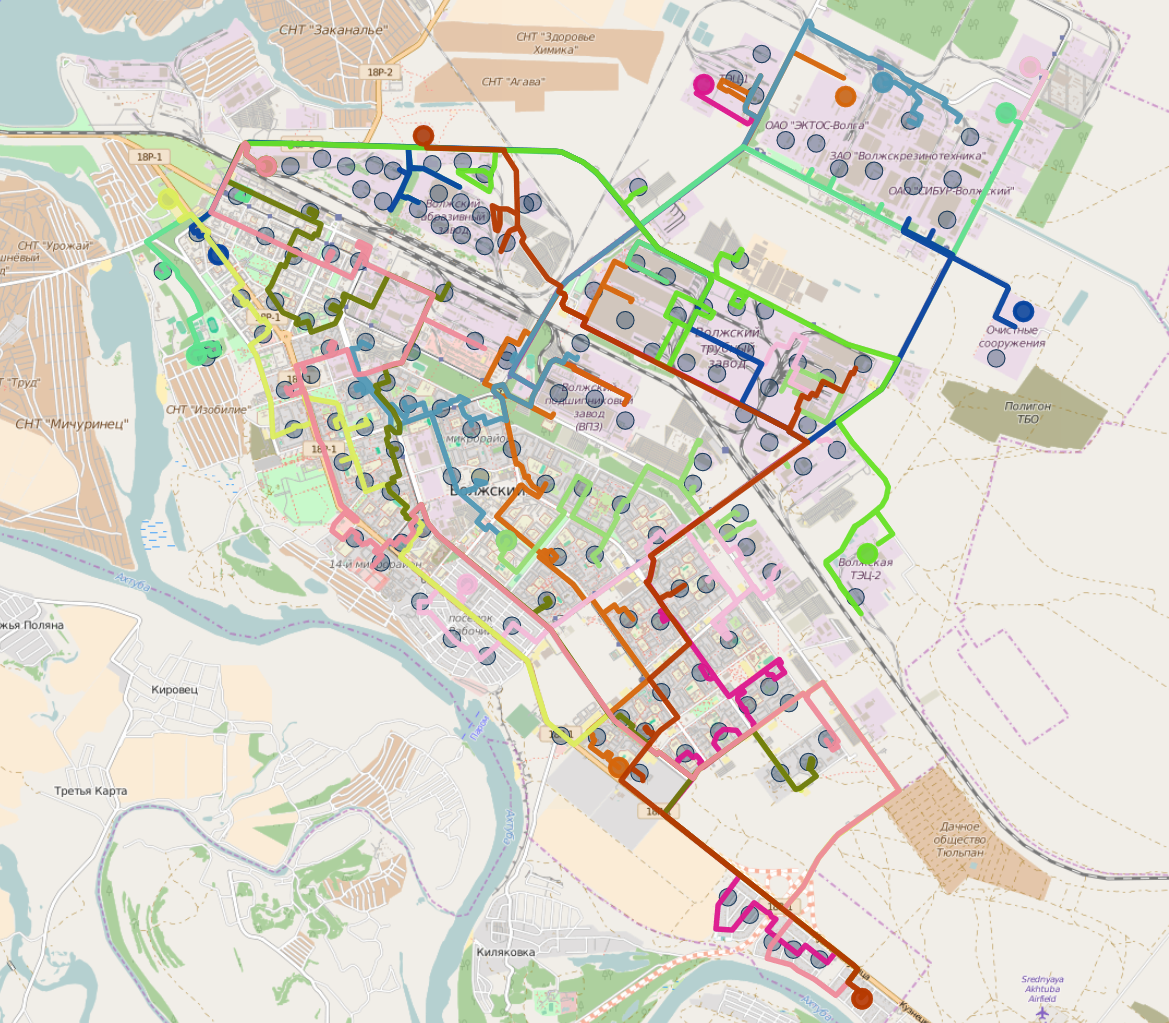
\includegraphics[width=0.8\textwidth]{200-12}
    \caption{Использование метрики OSRM для 200 кластеров и 12 маршрутов.}
    \label{fig:network-02b}
\end{figure}

\begin{figure}[ht!]
    \centering
    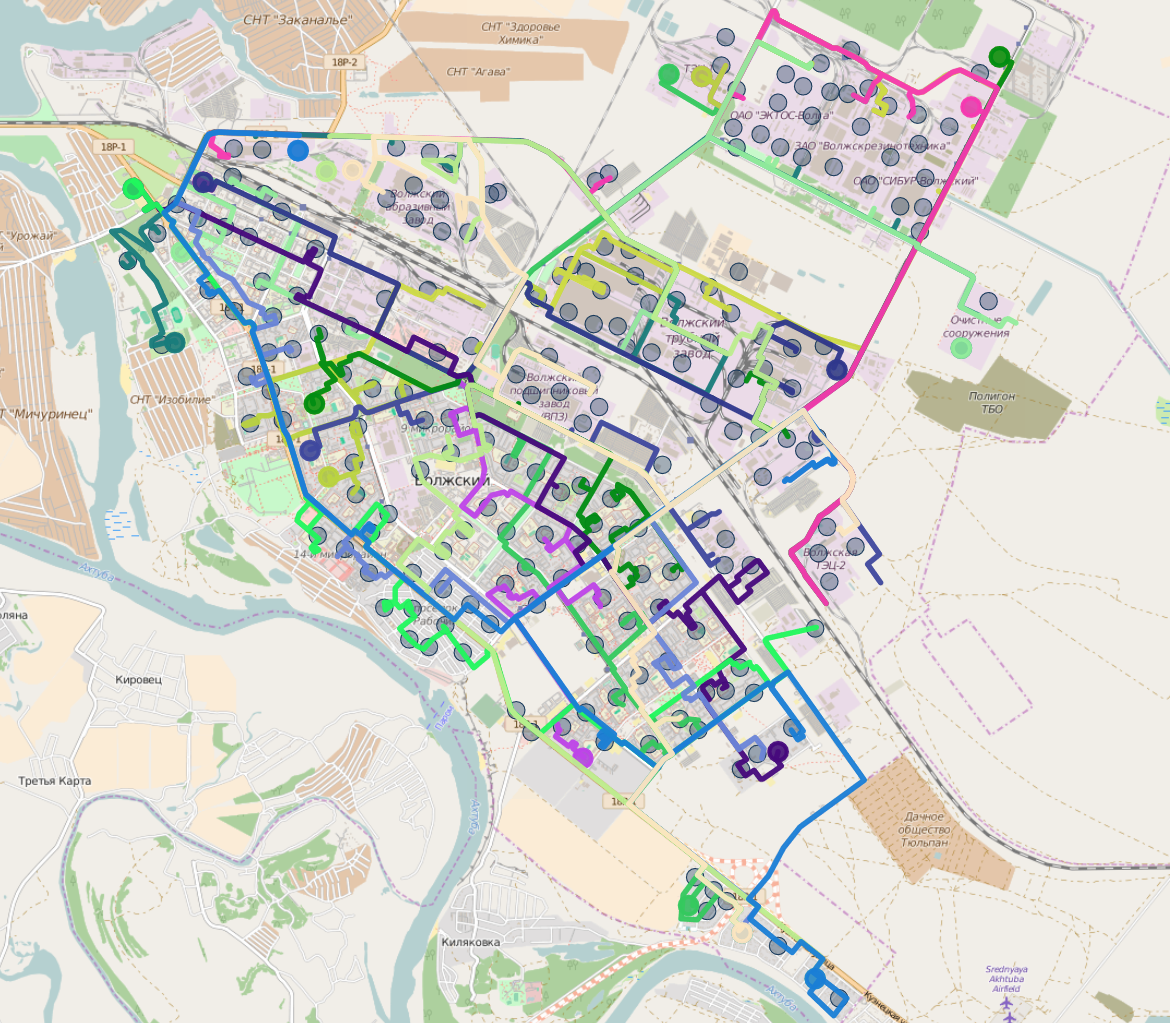
\includegraphics[width=0.8\textwidth]{300-16}
    \caption{Использование метрики OSRM для 300 кластеров и 16 маршрутов.}
    \label{fig:network-02c}
\end{figure}

\clearpage

\begin{table}[ht!]
    \centering
    \caption{Результаты эксперимента алгоритма из пункта \ref{sec:second_alg}.\\
        Данные представлены в формате минуты:секунды.}
    \label{table-time-results}
    \small
    \begin{tabular}{|c|l|c|c|c|c|c|c|l|l|l|c|}
        \hline
        \multicolumn{1}{|l|}{}      &          & \multicolumn{10}{c|}{количество маршрутов}                                                                                                       \\ \hline
        \multicolumn{1}{|l|}{узлы} & стратегия & 8     & 10    & 12    & 14    & 16    & 18    & \multicolumn{1}{c|}{40} & \multicolumn{1}{c|}{60} & \multicolumn{1}{c|}{80} & 100  \\ \hline
        \multirow{3}{*}{100}        & graph    & 0:06  & 0:04  & 0:03  & 0:03  & 0:02  & 0:02  & 0:01                    & 0:01                    & 0:01                    & 0:01 \\ \cline{2-12} 
        & S. OSRM  & 3:22  & 2:35  & 2:01  & 1:44  & 1:40  & 1:29  & 0:17                    & 0:23                    & 0:25                    & 0:29 \\ \cline{2-12} 
        & P. OSRM  & 1:11  & 1:03  & 0:51  & 0:50  & 0:42  & 0:42  & 0:25                    & 0:17                    & 0:34                    & 0:37 \\ \specialrule{.05em}{.02em}{.02em}
        \multirow{3}{*}{150}        & graph    & 0:16  & 0:12  & 0:10  & 0:08  & 0:07  & 0:07  & 0:04                    & 0:03                    & 0:02                    & 0:03 \\ \cline{2-12} 
        & S. OSRM  & 9:32  & 7:24  & 6:06  & 5:34  & 4:59  & 4:15  & 1:27                    & 1:06                    & 0:57                    & 1:13 \\ \cline{2-12} 
        & P. OSRM  & 2:39  & 2:17  & 1:58  & 1:56  & 1:42  & 1:41  & 1:06                    & 1:13                    & 0:56                    & 1:02 \\ \specialrule{.05em}{.02em}{.02em}
        \multirow{3}{*}{200}        & graph    & 0:40  & 0:31  & 0:25  & 0:20  & 0:20  & 0:16  & 0:08                    & 0:06                    & 0:05                    & 0:05 \\ \cline{2-12} 
        & S. OSRM  & 29:33 & 22:45 & 18:36 & 16:43 & 13:53 & 11:35 & 3:18                    & 2:20                    & 2:12                    & 2:47 \\ \cline{2-12} 
        & P. OSRM  & 6:51  & 5:23  & 5:06  & 4:07  & 3:48  & 3:38  & 2:08                    & 1:53                    & 1:49                    & 2:06 \\ \specialrule{.05em}{.02em}{.02em}
        \multirow{3}{*}{300}        & graph    & 1:38  & 1:16  & 1:02  & 0:51  & 0:46  & 0:40  & 0:20                    & 0:14                    & 0:11                    & 0:11 \\ \cline{2-12} 
        & S. OSRM  & 48:20 & 35:24 & 30:00 & 27:17 & 21:06 & 18:01 & 8:41                    & 6:02                    & 6:21                    & 6:57 \\ \cline{2-12} 
        & P. OSRM  & 16:20 & 12:28 & 10:31 & 9:08  & 8:35  & 7:35  & 4:38                    & 4:19                    & 4:46                    & 4:20 \\ \hline
    \end{tabular}
\end{table}

\clearpage

\section{Обсуждение результатов}
% TODO

% полный треш по тексту
% На основе результатов алгоритма \ref{alg:min-length} можно выделить следующие особенности: (I) анализ 
% эффективности различных стратегий реализации; (II), как производительность зависит от заранее определенного 
% числа узлов в сети; (III), как производительность (с точки зрения сложности времени) зависит от заранее 
% определенного количества маршрутов в сети; (IV) есть ли оптимальные узлы пара -- маршруты относительно 
% времени расчета; (V) общая длина окончательной сети.

Таблица \ref{table-time-results} показывает результаты реализации используемого алгоритма для различных 
стратегий с точки зрения времени расчёта. Стратегия, помеченная как "graph" -- последовательная реализация, 
"S.OSRM" -- последовательная реализация с использованием OSRM и "P.OSRM" -- параллельной реализации OSRM соответственно.

% По таблице \ref{table-time-results} можно видеть, что скорость 
% расчёта параллельной версии над последовательной на малом числе маршрутов является колосальной, в то время 
% как на большом количестве маршрутов -- минимальна. Это объясняется тем, что за одну итерацию алгоритма 
% происходит исключение узлов из рассмотрения равное числу маршрутов \( n_r \), т.е. чем больше число маршрутов 
% в сети, тем быстрее происходит распределение узлов графа по данным маршрутам.

\section{Заключение}
% TODO
    \chapter*{}
\begin{center}
	ЗАКЛЮЧЕНИЕ
\end{center}
\addcontentsline{toc}{chapter}{Заключение}

    \renewcommand{\bibname}{СПИСОК ИСПОЛЬЗУЕМЫХ ИСТОЧНИКОВ}
\addcontentsline{toc}{chapter}{Список используемых источников}

\begin{thebibliography}{10}
    \bibitem{bib:6} Suhl,~H. Bardeen-cooper-schrieffer theory of 
        superconductivity in the case of overlapping bands~/ H.~Suhl, 
        B.~T. Matthias, L.~R. Walker~// Physical Review Letters. "--- 
        1959. "--- V.~3. --- P.~552--554.

    \bibitem{bib:7} Liu,~A.~Y. Beyond eliashberg superconductivity in 
        \( \mathrm{MgB_2} \): Anharmonicity, Two-Phonon Scattering, and 
        Multiple Gaps~/ A.~Y. Liu, I.~I. Mazin, J.~Kortus~// 
        Physical Review Letters. "--- 2001. "--- V.~87. "--- P.~087005.

    \bibitem{bib:8} Gurevich,~A. Enhancement of the upper critical field by 
        nonmagnetic impurities in dirty two-gap superconductors~/ 
        A.~Gurevich~// Physical Review B. "--- 2003. "--- V.~67. "--- 
        P.~184515.

    \bibitem{bib:9} Type-1.5 superconductivity in multiband systems: 
        Magnetic response, broken symmetries and microscopic theory - 
        A brief overview~/ E.~{Babaev} [et~al]~// 
        Physica C Superconductivity. "--- 2012. "--- V. 479. "--- 
        P.~2--14.

    \bibitem{bib:10} Zhitomirsky,~M.~E. Ginzburg-landau theory of vortices in 
        a multigap superconductor~/ M.~E. Zhitomirsky, V.~H. Dao~// 
        Physical Review B. "--- V.~69. "--- P.~054508.

    \bibitem{bib:11} Ishida,~K. To what extent iron-pnictide new 
        superconductors have been clarified: A Progress Report~/ 
        K.~Ishida, Y.~Nakai, H.~Hosono~// 
        Journal of the Physical Society of Japan. "--- 2009. "--- V.~78, 
        №~6. "--- P.~062001.

    \bibitem{bib:12.1} Ashcroft,~N.~W. Hydrogen dominant metallic alloys: 
        High Temperature Superconductors?~/ N.~W. Ashcroft~// 
        Physical Review Letters. "---2004. "--- V.~92. "--- P.~187002.

    \bibitem{bib:12.2} Moulopoulos,~K. Generalized coulomb pairing in the 
        condensed state~/ K.~Moulopoulos, N.~W. Ashcroft~// 
        Physical Review Letters. "--- 1991. "--- V.~66. "--- P.~2915--2918.

    \bibitem{bib:13} Vortex sublattice melting in a two-component 
        superconductor~/ E.~Sm\o{}rgrav, J.~Smiseth, E.~Babaev, A.~Sudb\o{}~// 
        Physical Review Letters. "--- 2005. "--- V.~94. "--- P.~096401.

    \bibitem{bib:14} Herland,~E.~V. Phase transitions in a three dimensional 
        \( \mathrm{U(1)\times U(1)} \) lattice london superconductor: 
        Metallic superfluid and charge-4e superconducting states~/ 
        E.~V. Herland, E.~Babaev, A.~Sudb\o{}~// Physical Review B. "--- 
        2010. "--- V.~82. "--- P.~134511.

    \bibitem{bib:3} Abrikosov,~A.~A. On the magnetic properties of 
        superconductors of the second group~/ A.~A. Abrikosov~// 
        Journal of Experimental and Theoretical Physics. "--- 1957. "---
        V.~5, №~6. "--- P.~1442--1452.

    \bibitem{bib:net} Ерин,~Ю. Сверхпроводимость 1,5-го рода: 
        ни два, ни полтора [Электронный ресурс] // 
        Научно-популярный проект <<Элементы>>. "--- Режим доступа: 
        \url{http://elementy.ru/news/431450} (дата обращ. 05.02.2014).

    \bibitem{ginzburg} Гинзбург,~В.~Л. Ферромагнитные сверхпроводники~/ 
        В.~Л. Гинзбург~// Журнал экспериментальной и теоретической физики. "---
        1956. "--- Т.~31. "--- С.~202--210.

    \bibitem{buzdin} Буздин,~А.~И. Существование сверхпроводящих стенок в 
        ферромагнетике~/ А.~И. Буздин, Л.~Н. Булаевский, С.~В. Панюков~// 
        Журнал экспериментальной и теоретической физики. "--- 1984. "---
        Т.~87. "--- С.~299--309.

    \bibitem{bulaev} Coexistence of superconductivity and magnetism. 
        Theoretical predictions and numerical results~/ L.~N. Bulaevskii, 
        A.~I. Buzdin, M.~L. Kulic, S.~V. Panyukov~// Advances in Physics. "---
        1985. "--- V.~34, №~2. "--- P.~175--261.

    \bibitem{shubnikov} Магнитные свойства сверхпроводящих металлов и 
        сплавов~/ Л.~В. Шубников, В.~И. Хоткевич, Ю.~Д. Шепелев, 
        Ю.~Н. Рябин~// Журнал экспериментальной и теоретической физики. "---
        1937. "--- Т.~7, №~2. "--- С.~221--237.

    \bibitem{ginzburg-landau} Гинзбург,~В.~Л. К теории сверхпроводимости~/
        В.~Л. Гинзбург, Л.~Д. Ландау~// Журналэкспериментальной и теоретической
        физики. "--- 1950. "--- Т.~20. "--- С.~1064.

    \bibitem{abrikosov} Абрикосов,~А.~А. О магнитных свойствах 
        сверхпроводников второй группы~/ А.~А. Абрикосов~// 
        Журнал экспериментальной и теоретической физики. "--- 1957. "---
        Т.~32, №~6. "--- С.~1442--1452.

    \bibitem{bib:1} Babaev,~E. Semi-meissner state and neither type-i nor 
        type-ii superconductivity in multicomponent superconductors~/ 
        E.~Babaev, M.~Speight~// Physical Review B. "--- 2005. "---
        V.~72. "--- P.~180502.

    \bibitem{bib:2} Babaev,~E. Type-1.5 superconducting state from an 
        intrinsic proximity effect in two-band superconductors~/ 
        E.~Babaev, J.~Carlstr\"om, M.~Speight~// Physical Review Letters. "---
        2010. "--- V. 105. "--- P.~067003.

    \bibitem{bib:16} Type-1.5 superconductivity~/ V.~Moshchalkov [et~al]~// 
        Physical Review Letters. "--- 2009. "--- V. 102. "--- P.~117001.

    \bibitem{bib:17} Scanning squid microscopy of vortex clusters in multiband 
        superconductors~/ T.~Nishio [et~al]~// Physical Review B. "---
        2010. "--- V.~81. "--- P.~020506.

    \bibitem{bib:main} Carlstr\"om,~J. Type-1.5 superconductivity in multiband 
        systems: Effects of interband couplings~/ J.~Carlstr\"om, E.~Babaev, 
        M.~Speight~// Physical Review B. "--- 2011. "--- V.~83. "--- 
        P.~174509.

    \bibitem{bib:superconductors} Коган,~Н.~Н. Сверхпроводимость 
        [Электронный ресурс] // Электронный каталог Science \& Technology. "---
        Режим доступа: 
        \url{http://www.science-techno.ru/nt/article/sverkhprovodimost} 
        (дата обращ. 05.02.2014).

    \bibitem{bib:19} Speight,~J.~M. Static intervortex forces~/ 
        J.~M. Speight~// Physical Review D. "--- 1997. "--- V.~55. "--- 
        P.~3830--3835.

    \bibitem{bib:20} Plohr,~B. The behavior at infinity of isotropic vortices 
        and monopoles~/ B.~Plohr, J.~Math~// 
        Journal of Mathematical Physics. "--- 1981. "--- V.~22. "--- 
        P.~2184--2190.

    \bibitem{bib:methods} Методы оптимизации: для студентов высших технических 
        учебных заведений~/ А.~В. Аттетков, С.~В. Галкин, В.~С. Зарубин, 
        А.~П. Крищенко. Математика в техническом университете. "--- 
        Москва : МГТУ им. Н. Э. Баумана, 2003. "--- С.~440.

    \bibitem{skajaa2010limited} Skajaa,~A. Limited memory BFGS for nonsmooth 
        optimization // Master's thesis. "--- 2010.

    \bibitem{bib:minimization} Carlstrom,~J. Unconventional states due to 
        non-pairwise intervortex interactions in multicomponent 
        superconductors [Electronic resource]~/ Available at: 
        \url{http://people.umass.edu/garaud/NonPairwise_files/%
            NumericalMethod3.pdf}.
\end{thebibliography}

\newpage
    % главы приложения
    \APPENDIX{Приложение А}{Техническое задание}

\thispagestyle{empty}
\begin{center}
    Министерство образования и науки Российской Федерации \\
    Федеральное государственное бюджетное образовательное учреждение высшего образования\\
    <<Волгоградский государственный технический университет>>\\
    Факультет электроники и вычислительной техники\\
    Кафедра <<Системы автоматизированного проектирования и поискового конструирования>>
    \vspace{1em}
\end{center}
\begin{flushright}
    \begin{center}
        \hspace*{10.5em}Утверждаю
    \end{center}
    И.о.зав. кафедрой <<САПР~и~ПК>>\\
    \UNDER{\LINE{3cm}}{\TINY{(подпись)}}\quad\UNDER{Щербаков~М.~В.}{\TINY{(инициалы, фамилия)}}\\
    <<\underline{\hspace{2em}}>> \underline{\hspace{7.5em}} \the\year\ г.
\end{flushright}
\begin{center}
    Программа формирования маршрутов общественного транспорта на основании обработки данных\\
    ТЕХНИЧЕСКОЕ ЗАДАНИЕ\\
    \vspace{2em}
    ВРБ.40461806.10.27-\SPECIFICATION.11-91\\
    ЛИСТОВ \SPAGES
\end{center}
\vspace{5em}
\begin{minipage}[t]{0.6\textwidth}
    \vspace{4em}
    \begin{flushleft}
        Нормоконтролер\\
        Садовникова~Н.~П.\\
        <<\LINE{1.5em}>>\ \LINE{7em} \the\year\ г.
    \end{flushleft}
\end{minipage}
\begin{minipage}[t]{0.39\textwidth}
    \begin{flushleft}
        Научный руководитель\\
        \underline{\smash{М.~В.~Щербаков\hspace{6em}}}\\
        <<\LINE{1.5em}>>\ \LINE{7em} \the\year\ г.\\
        Исполнитель\\
        Студент группы\\
        \underline{\smash{А.~В.~Голубев\hspace{7em}}}\\
        <<\LINE{1.5em}>>\ \LINE{7em} \the\year\ г.\\
    \end{flushleft}
\end{minipage}
\vspace{\fill}
\begin{center}
    Волгоград \the\year\ г.
\end{center}
\newpage

% конец содержания для ПЗ
\stopcontents

\tocless\part{Аннотация}
Документ содержит задание на разработку системы <<Программа формирования маршрутов общественного транспорта 
на основании обработки данных>> для автоматизации построения маршрутов общественного транспорта. В документе 
дано общее описание системы, её название, цель создания и назначение. Приведено описание основных требований 
предъявляемых к системе в целом и функциям системы, на основе которых выделены и описаны подсистемы. 
Разработана предварительная структура разрабатываемой системы. Описаны основные алгоритмы, которые будут 
использованы.
\newpage

% содержание для ТЗ
\startcontents[sections]
\printcontents[sections]{ }{2}{\contentsname}
% обнуляем счётчик глав
\setcounter{chapter}{0}
\begingroup

\makeatletter
\renewcommand\chapter{\par%
  \thispagestyle{plain}%
  \global\@topnum\z@
  \@afterindentfalse
  \secdef\@chapter\@schapter}
\makeatother

\newpage

% ТЗ ГОСТ 34
% http://www.rugost.com/index.php?option=com_content&view=article&id=108:34-4-8&catid=25&Itemid=62
% http://www.prj-exp.ru/gost/gost_34-602-89.php

\chapter{Общие сведения}
\section{Полное наименование системы и её условное обозначение}
Полное наименование системы -- <<Программа формирования маршрутов 
общественного транспорта на основании обработки данных>>.

Краткое наименование системы -- <<АС>>. В дальнейшем просто -- система.

\section{Шифр темы или шифр (номер) договора}
Тема работы: <<Разработка эволюционного алгоритма формирования маршрутов 
общественного транспорта на основании обработки данных>>

\section{Перечень документов, на основании которых создается система}
Основанием для проведения работ по созданию системы является задание приказ \ldots

\section{Наименование предприятий (объединений) разработчика и заказчика (пользователя)}
Заказчик -- Волгоградский государственный технический университет.\\
Исполнитель -- студент группы САПР-2п1 Голубев Алексей.

\section{Плановые сроки начала и окончания работы по созданию системы}
Начало разработки -- 01.10.2015 г.\\
Окончание разработки -- 31.05.2016 г.

\section{Порядок оформления и предъявления заказчику результатов работ по созданию системы}
Система передаётся в виде исходных кодов на языке Python в установленные сроки по созданию системы.
Приемка системы осуществляется комиссией в составе уполномоченных представителей Заказчика и Исполнителя. 
Порядок предъявления системы, ее испытаний и окончательной приемки определен в разделе \ref{sec:acceptance} 
настоящего ТЗ. Одновременно с предъявлением системы производится сдача разработанного Исполнителем комплекта 
документации согласно разделу \ref{sec:document} настоящего ТЗ.

\vspace{3em}
\chapter{Назначение и цели создания (развития) Системы}
\section{Назначение Системы}
Система предназначена для формирования начальной маршрутной сети общественного транспорта на основе 
кластеризованных данных о перемещении.

\section{Цели создания Системы}
Автоматизация процесса построения маршрутной сети общественного транспорта.

\vspace{3em}
\chapter{Характеристика объекта автоматизации}
\section{Краткие сведения об объекте автоматизации или ссылки на документы, содержащие такую информацию}
В ходе проведения работ по разработке Системы автоматизируются процессы построения маршрутов общественного 
транспорта. Система будет эксплуатироваться на персональном компьютере по выбору Исполнителя.

\section{Сведения об условиях эксплуатации объекта автоматизации}
Система должна быть рассчитана на эксплуатацию в составе программно– технического комплекса и учитывать 
разделение ИТ инфраструктуры на внутреннюю и внешнюю. Для нормальной эксплуатации разрабатываемой системы 
должно быть обеспечено бесперебойное питание ПЭВМ. При эксплуатации система должна быть обеспечена 
соответствующая стандартам хранения носителей и эксплуатации ПЭВМ температура и влажность воздуха. 
Периодическое техническое обслуживание используемых технических средств должно проводиться в соответствии 
с требованиями технической документации изготовителей, но не реже одного раза в год. В процессе проведения 
периодического технического обслуживания должны проводиться внешний и внутренний осмотр и чистка 
технических средств, проверка контактных соединений, проверка параметров настроек работоспособности 
технических средств и тестирование их взаимодействия.

Объектом автоматизации является формирование маршрутов общественного транспорта.

\vspace{3em}
\chapter{Требования к системе}
\section{Требования к системе в целом}
Общими требованиями к автоматизированной системе являются:
\begin{itemize}
    \item система должна иметь модульную архитектуру и высокую степень в масштабировании;
    \item система должна использовать методы параллельного программирования.
\end{itemize}

Основными принципами создания Системы являются:
\begin{itemize}
    \item использование современного программного и аппаратного обеспечения;
    \item высокая степень масштабирования программных и аппаратных средств.
\end{itemize}

\section{Требования к структуре и функционированию системы}
В состав Системы должны входить следующие подсистемы
\begin{enumerate}
    \item Подсистема построения и расчёта длины маршрута;
    \item Подсистема генерации маршрутной сети;
    \item Подсистема сохранения, загрузки и преобразования данных.
\end{enumerate}

\subsection{Перечень подсистем, их назначение и основные характеристики}
Подсистема построения и расчёта длины маршрута предназначена для:
\begin{itemize}
    \item взаимодействия с программных обеспечение OSRM;
    \item построения маршрута проходящего через контрольные точки;
    \item расчёта длины построенного маршрута.
\end{itemize}

Подсистема генерации маршрутной сети предназначена для:
\begin{itemize}
    \item инициализации маршрутной сети;
    \item нахождения терминальных кластеров;
    \item построения маршрутной сети по заданной метрике.
\end{itemize}

Подсистема сохранения, загрузки и преобразования данных предназначена для:
\begin{itemize}
    \item загрузки кластеризованных данных о перемещении;
    \item преобразованию загруженных данных;
    \item сохранения расчётных данных для последующей обработки.
\end{itemize}

\section{Требования к режимам функционирования системы}
Для АС определены следующие режимы функционирования:
\begin{itemize}
    \item Нормальный режим функционирования;
\end{itemize}
В нормальном режиме функционирования системы:
\begin{itemize}
    \item клиентское программное обеспечение и технические средства пользователей системы 
        обеспечивают возможность круглосуточного функционирования;
    \item исправная работа оборудования, составляющее комплекс технических средств;
    \item исправное функционирует системных и прикладного программного обеспечение системы.
\end{itemize}
Для обеспечения нормального режима функционирования системы необходимо выполнять требования и 
выдерживать условия эксплуатации программного обеспечения и комплекса технических средств системы, 
указанные в соответствующих технических документах (техническая документация и т.д.).

\section{Требования по диагностированию системы}
Система должна удовлетворять следующим требованиям по диагностированию:
\begin{itemize}
    \item запись при возникновении системных ошибок в ходе выполнения работы в системный журнал;
    \item журналирование работы подсистем;
    \item выдача пользователю сообщений, содержащих адекватное описание нарушения 
        работоспособности.
\end{itemize}

\section{Перспективы развития, модернизации системы}
Для приведения Системы к готовности для эксплуатации по результатам работы могут быть 
проведены работы в следующих направлениях:
\begin{itemize}
    \item масштабируемость системы за счёт вынесения функций в отдельные модули с 
        последующей структуризацией;
    \item создания модификаций на основе системы (замена используемых метрик, логических 
        структур и т.п.);
    \item адаптации логики работы системы к изменениям в документах, регламентирующих 
        деятельность Заказчика.
\end{itemize}

\section{Требования к надежности}
Надежное (устойчивое) функционирование программы должно быть обеспечено выполнением совокупности 
организационно-технических мероприятий, перечень которых приведен ниже: 
\begin{itemize}
    \item использованием лицензионного программного обеспечения; 
    \item использованием нового программного обеспечения;
    \item использованием отказоустойчивого оборудования;
    \item соблюдение сохранности входных данных.
\end{itemize}

\section{Требования к эргономике и технической эстетике}
Требования к пользовательскому интерфейсу не специфицируются.

\section{Требования к эксплуатации, техническому обслуживанию, ремонту и хранению компонентов системы}
Требования к эксплуатации, техническому обслуживание, ремонту и хранению компонентов системы 
не предъявляются.

\section{Требования к защите информации от несанкционированного доступа}
Обеспечение требований по защите информации от несанкционированного доступа возлагается на систему 
безопасности операционной системы.

\section{Требования по сохранности информации при авариях}
Для сохранности информации при авариях в качестве компонентов технических средств организацией должны 
использоваться только высококачественные комплектующие и технические средства с высоким значением времени 
наработки на отказ (до отказа).

Требования надежности работы в целом и сохранности информации во время аварии должны быть учтены при выборе 
аппаратного обеспечения и квалификации обслуживающего персонала.

\section{Требования к видам обеспечения}
\subsection{Информационное обеспечение системы}
Технические средства, обеспечивающие хранение информации, должны использовать современные 
технологии, позволяющие обеспечить повышенную надежность хранения данных и оперативную замену 
оборудования (распределенная избыточная запись/считывание данных; зеркалирование; независимые 
дисковые массивы; кластеризация). Подсистемы должны работать только со своими структурами данных.

\subsection{Программное обеспечение системы}
\label{sec:software}
В Системе должны максимально использоваться программные продукты с открытой лицензией. 

Используемые программные продукты:
\begin{itemize}
    \item Python 3 -- высокоуровневый язык программирования общего назначения, ориентированный на повышение 
        производительности разработчика и читаемости кода;
    \item JavaScript -- прототипно-ориентированный сценарный язык программирования;
    \item Leaflet -- библиотека для отображения карт на веб-сайтах;
    \item Geographiclib -- библиотека для работы с географическими данными;
    \item Polyline -- библиотека для декодирования геоинформационных данных;
    \item Requests -- библиотека для работы с HTTP-запросами;
    \item Numpy -- библиотека высокоуровневых математических функций;
    \item Geojson -- библиотека сериализации данных.
\end{itemize}

Реализация программных модулей должна соответствовать текущим требованиям оформления программного кода 
с открытой лицензией. Среди которых:
\begin{itemize}
    \item Форматирование кода в соответствии с PEP;
    \item Комментирование программного кода;
    \item Переносимость программного кода;
\end{itemize}

\subsection{Требования к лингвистическому обеспечению системы}
Для лингвистического обеспечения системы приводятся требования к применению в системе языков программирования 
высокого уровня, а также требования к кодированию и декодированию данных.

Должны выполняться следующие требования к кодированию и декодированию данных: UTF-8 для подсистемы хранения 
данных; UTF-8 информации, поступающей из систем-источников.

\subsection{Требования к языку программирования}
Языком программирования должен быть выбран -- Python 3. К среде разработки особых требований не предъявляется.

\subsection{Техническое обеспечение системы}
\subsubsection{Требования к программному обеспечению системы}
Программное обеспечение системы должно быть достаточным для выполнения всех реализуемых функций системы, а 
также иметь средства организации всех требуемых процессов обработки данных, позволяющих своевременно 
выполнять все автоматизируемые функции во всех регламентных режимах функционирования системы. Необходимый 
набор программных средств для работы системы должен быть следующим:
\begin{itemize}
    \item операционная система поддерживающая установку интерпретатора Python;
    \item интерпретатор языка Python не ниже 3;
    \item библиотеки из пункта \ref{sec:software}.
\end{itemize}

\subsection{Требования к техническому обеспечению системы}
Система должна функционировать на аппаратном обеспечении, на котором может быть запущено клиентское 
программное обеспечение, но для достижения оптимальной производительности необходима конфигурация приведенная 
ниже:
\begin{itemize}
    \item Многоядерный процессор не менее 2 ГГц;
    \item Не менее 4 Гб оперативной памяти;
    \item По крайней мере, 100 Мб свободного места на диске.
\end{itemize}

\subsection{Требования к математическому обеспечению}
При выборке и разработке моделей, методов и алгоритмов необходимо учитывать следующие требования:
\begin{itemize}
    \item Универсальность;
    \item Алгоритмическая надёжность.
\end{itemize}

Разделы математического обеспечения требуемые для реализации:
\begin{itemize}
    \item Линейная алгебра;
    \item Разделы тригонометрии и геометрии.
\end{itemize}

Разделы информатики требуемые для реализации:
\begin{itemize}
    \item Теория алгоритмов;
    \item Алгоритмы и структуры данных;
    \item Прикладная информатика;
    \item Компьютерное моделирование и численные методы;
    \item Распределенные вычисления;
    \item Интеллектуальны Анализ данных.
\end{itemize}

\subsubsection{Эксплуатационные требования}
Особых эксплуатационных требований к Системе не предъявляется.

\vspace{3em}
\chapter{Состав и содержание работ по созданию (развитию) системы}
Проектирование системы должно происходить следующим образом:
\begin{itemize}
    \item разработка, согласование и утверждение технического задания по ГОСТ 34.602-89 на 
        проектирование -- 3 недели;
    \item разработка рабочего проекта программы -- 10 недель.
\end{itemize}

Этап рабочего проекта разбивается на следующие под этапы:
\begin{itemize}
    \item разработка и отладка программы -- 4 недели;
    \item разработка программной документации -- 3 недели;
    \item испытания программы -- 3 недели.
\end{itemize}

Остальные сроки рассчитываются исходя из сроков утверждения ТЗ. Дата начала должна быть не позднее 
01.10.2015. Дата окончания работ не позднее 31.05.2016.

\vspace{3em}
\chapter{Порядок контроля и приемки Системы}
\label{sec:acceptance}
\section{Состав, объем и методы испытаний системы и ее составных частей}
Первая версия Системы должна пройти предварительные испытания, состоящие из функционального тестирования. 
Будут проведены испытания работы модулей системы с целью сбора перечня предложений и выявления недостатков. 

\section{Общие требования к приемке работ}
В процессе приёмки работ должна быть осуществлена проверка Системы на соответствии требованиям настоящего 
<<Технического задания>>.

В процессе приёмочных испытаний должен вестись журнал, в котором будут фиксироваться результаты выполненных 
работ, замечания по работе программного обеспечения и предложения по изменению работы программного 
обеспечения.

По результатам испытаний возможны доработки и исправления. Выявленные в ПО и документации недостатки 
Исполнитель исправляет за свой счёт в специально оговоренные после проведения испытаний сроки.

\vspace{3em}
\chapter{Требования к документированию}
\label{sec:document}
В состав программной документации, сопровождающей проектируемое изделие должны входить следующие документы:
\begin{enumerate}
    \item Пояснительная записка к техническому проекту;
    \item техническое задание;
\end{enumerate}

\endgroup
\stopcontents[sections]
\end{document}
